% For TeXworks
\makeatletter
\declare@file@substitution{revtex4-1.cls}{revtex4-2.cls}
\makeatother

% Define document class
\documentclass[twocolumn,twocolappendix,linenumbers]{aastex631}
% \documentclass[linenumbers]{aastex631}

% \usepackage{showyourwork}
\usepackage{amsmath}
\usepackage{amssymb}
\usepackage{graphicx}
% \usepackage{layouts}
\usepackage{xcolor}
% \usepackage{upgreek}
\let\tablenum\relax
\usepackage{siunitx}
\usepackage{xspace}
% Dropped capital
\usepackage{lettrine}

% ***Fancy*** dropped capital
\input Zallman.fd
\renewcommand{\LettrineFontHook}{\usefont{U}{Zallman}{xl}{n}}
\setcounter{DefaultLines}{3} % number of lines dropped capital should take up

% user-defined commands
\newcommand{\vice}{{\tt VICE}\xspace}
\newcommand{\todo}[1]{{\color{red}#1}}
\newcommand{\osuaffil}{Department of Astronomy, The Ohio State University, 140 W. 18th Ave, Columbus OH 43210, USA}
\newcommand{\ccappaffil}{Center for Cosmology and AstroParticle Physics, The Ohio State University, 191 W. Woodruff Ave., Columbus OH 43210, USA}
\newcommand{\aFe}{[$\alpha$/Fe]\xspace}
\newcommand{\mathXH}{{\rm [X/H]}}
\newcommand{\mathOH}{{\rm [O/H]}}
\newcommand{\mathFeH}{{\rm [Fe/H]}}
\newcommand{\mathOFe}{{\rm [O/Fe]}}
\newcommand{\mathaFe}{[\alpha/{\rm Fe}]}
\newcommand{\yZ}[1]{$y/Z_\odot=#1$}
\newcommand{\kpc}{\,{\rm kpc}}
\newcommand{\Gyr}{\,{\rm Gyr}}
\newcommand{\dex}{\,{\rm dex}}
\newcommand{\Msun}{\,{\rm M}_\odot}
\newcommand{\kms}{\,{\rm km}\,{\rm s}^{-1}}
\newcommand{\onecolumn}{0.47\textwidth}

% Citation aliases
\defcitealias{johnson_stellar_2021}{J21}
\defcitealias{leung_variational_2023}{L23}
\defcitealias{dubay_galactic_2024}{D24}

\shorttitle{Two-Infall in VICE}
\shortauthors{Dubay et al.}
% \linespread{1.8}

\begin{document}

% Title
\title{Challenges to the Two-Infall Scenario by Large Stellar Age Catalogs}

% Author list
% \author[]{Amanda Ash}
\author[0000-0003-3781-0747]{Liam O.\ Dubay}
\affiliation{\osuaffil}
\affiliation{\ccappaffil}
\author[0000-0001-7258-1834]{Jennifer A.\ Johnson}
\affiliation{\osuaffil}
\affiliation{\ccappaffil}
\author[0000-0002-6534-8783]{James W.\ Johnson}
\affiliation{Observatories of the Carnegie Institution for Science, 813 Santa Barbara St., Pasadena CA 91101, USA}
% \affiliation{\osuaffil}
% \affiliation{\ccappaffil}
\author[0000-0002-2854-5796]{John D.\ Roberts}
\affiliation{\osuaffil}
\affiliation{\ccappaffil}
% \author[0000-0001-7775-7261]{David H. Weinberg}
% \author{coauthors}

\correspondingauthor{Liam O.\ Dubay}
\email{dubay.11@osu.edu}

\begin{abstract}
    Stars in the Milky Way disk exhibit a clear separation into two chemically distinct populations based on their [$\alpha$/Fe] ratios. This $\alpha$-bimodality is not a universal feature of simulated disk galaxies and may point to a unique evolutionary history. A popular explanation is the two-infall scenario, which postulates that two periods of substantial accretion rates dominate the assembly history of the Galaxy. 
    % However, most previous studies using the two-infall scenario have explored a limited portion of the parameter space, typically neglecting radial migration and assuming that the Galactic disk never ejected a substantial outflow. 
    Thanks to recent advances in stellar age measurements, we can now compare this popular model to more direct measurements of the Galaxy's evolutionary timescales across the disk. 
    % We run multi-zone galactic chemical evolution models with a two-infall-driven star formation history, radially dependent mass-loaded outflows, and a prescription for radial migration tuned to a hydrodynamical simulation. We compare our model results to abundance patterns across the disk from APOGEE DR17, supplemented with stellar age estimates through multiple methods. 
    We run multi-zone galactic chemical evolution models with a two-infall-driven star formation history and compare the results against abundance patterns across the disk from APOGEE DR17, supplemented with stellar ages estimated through multiple methods.
    Although the two-infall scenario offers a natural explanation for the $\alpha$-bimodality, it struggles to explain several features of the age--abundance structure in the disk. First, our models generically predict a massive and long-lasting dilution event, but the data show that stellar metallicity is remarkably constant across much of the lifetime of the disk. This apparent age-independence places considerable restrictions upon the two-infall parameter space. Second, most local metal-rich stars in APOGEE have intermediate ages, yet our models predict these stars should either be very old or very young. Some of these issues can be mitigated, but not completely resolved, by allowing the accreted gas to be pre-enriched to low metallicity. 
    % Restrictions upon the two-infall parameter space also limit the application of other merger-dominated star formation histories to the Milky Way.
    These restrictions also place limits on the role of merger events in shaping the chemical evolution of the thin disk in general.
\end{abstract}

\section{Introduction}
\label{sec:introduction}

% \todo{Hook, summary of alpha-bimodality.}
\lettrine{G}{alactic chemical evolution} (GCE) aims to explain the metal abundance patterns observed in the Milky Way (MW) by modeling the star formation history and evolution of the Galaxy. A long-standing paradigm of GCE is that the metallicity of the interstellar medium (ISM) increases over time due to supernova enrichment from successive generations of stars \citep[e.g.,][]{tinsley_stellar_1979,matteucci_relative_1986}. In this view, one feature of the MW disk that is difficult to explain is the so-called ``$\alpha$-bimodality'': the presence of two populations of stars at similar metallicity but separated by their \aFe ratio \citep[e.g.,][]{bensby_exploring_2014}. The high-$\alpha$ sequence consists of old stars \citep[$\gtrsim9$ Gyr; e.g.,][]{pinsonneault_apokasc-3_2025} with super-Solar \aFe and is associated with the kinematic thick disk \citep[e.g.,][]{fuhrmann_nearby_1998}, while the low-$\alpha$ sequence is younger, with approximately Solar \aFe, and is associated with the kinematic thin disk. The $\alpha$-bimodality is present across the Galactic disk, but the relative strength of the high- and low-$\alpha$ sequences varies by location \citep{hayden_chemical_2015}. 

An explanation for the MW $\alpha$-bimodality has yet to be broadly accepted in the GCE literature. An $\alpha$-bimodality is not a universal feature in simulated MW-mass galaxies \citep[e.g.,][]{mackereth_origin_2018,parul_effect_2025}, and tentatively does not exist in M31 (\citealt{nidever_prevalence_2024}; but see also \citealt{kobayashi_fe_2023}). Its presence and characteristics in our Galaxy could potentially have arisen to a unique evolutionary history. GCE models that attempt to solve this problem generally fall into two camps. Some explain the $\alpha$-bimodality as a result of secular processes, such as the radial migration of stars and the inside-out growth of the disk \citep[e.g.,][]{schonrich_chemical_2009,kubryk_evolution_2015,sharma_chemical_2021,chen_chemical_2023,prantzos_origin_2023}. Others argue for a bursty star formation history driven by multiple accretion events \citep[e.g.,][]{chiappini_chemical_1997,mackereth_origin_2018,spitoni_beyond_2023}.
% Studies of simulations have suggested that the $\alpha$-bimodality could be driven by clumpy star formation at high redshift \citep{clarke_imprint_2019}, a major gas-rich merger \citep{buck_origin_2020}, or re-accretion of metal-rich outflows \citep{khoperskov_bimodality_2021}.

% Summary of two-infall literature
The two-infall scenario was first proposed by \citet{chiappini_chemical_1997} to explain the origin of the high- and low-$\alpha$ disks. Though the model has since been refined, the basic premise remains the same: the rate of gas accretion onto the disk is described by two consecutive bursts that each decay with time. The relatively low infall rate between the two bursts causes star formation to slow down, allowing the gas abundance to evolve between the high- and low-$\alpha$ sequences while producing few stars in between. 
The infall timescale for the low-$\alpha$ disk can vary with radius to produce inside-out disk growth and a radial metallicity gradient \citep{romano_mass_2000}.
The initial model of \citet{chiappini_chemical_1997} successfully reproduced the available abundance data at the time, which were largely confined to the Solar neighborhood.

Subsequent studies refined the two-infall scenario to reproduce abundance data across the disk \citep[e.g.,][]{chiappini_abundance_2001,chiappini_oxygen_2003}. Others have explored the SN Ia delay-time distribution \citep{matteucci_effect_2009,palicio_analytic_2023}, galactic fountains \citep{spitoni_effects_2009}, radial gas flows \citep{spitoni_effects_2011,palla_chemical_2020}, variations in the star formation efficiency \citep{spitoni_effects_2011,palla_chemical_2020}, radial stellar migration \citep{spitoni_effect_2015,palla_mgfe_2022}, azimuthal abundance variations \citep{spitoni_2d_2019}, and pre-enriched gas infall \citep{palla_chemical_2020,spitoni_remind_2024}. \citet{spitoni_beyond_2023} and \citet{palla_mapping_2024} proposed a third gas accretion event in the last $\sim3$ Gyr to match the inferred star formation history from {\it Gaia} \citep{ruiz-lara_recurrent_2020} and to explain the recent abundance evolution (or lack thereof) in the Solar neighborhood. Most recently, \citet{hegedus_reconstructing_2025} constrained the infall timescales using chemical abundances for $\sim400,000$ stars from the 19th data release of the Sloan Digital Sky Survey (SDSS; \todo{Hawkins et al. 2025, in preparation}).

% \todo{Outflows.} 
While previous studies have explored a large parameter space, most have assumed that the Galactic disk never ejected a substantial outflow. This decision is based on hydrodynamic simulations of Galactic fountains ejected by CC SNe, which predict that ejected material falls back onto the disk on relatively short timescales \citep{spitoni_galactic_2008,spitoni_effects_2009} and close to their point of origin \citep{melioli_hydrodynamical_2008,melioli_hydrodynamical_2009}, suggesting that the effect on GCE should be minimal. However, the effects of feedback in simulations are sensitive to its implementation \citep[e.g.,][]{li_effects_2020,hu_code_2023}; other simulations of MW-like galaxies with different prescriptions do produce mass-loaded outflows \citep[e.g.,][]{brook_hierarchical_2011,gutcke_nihao_2017,nelson_first_2019,peschken_angular_2021,kopenhafer_seeking_2023}. Empirically, mass-loading has been observed in nearby starburst galaxies \citep[e.g.,][]{lopez_temperature_2020,cameron_duvet_2021,lopez_x-ray_2023} but not MW-like systems because the predicted column densities are below current detection limits \citep[see reviews by][]{veilleux_cool_2020,thompson_theory_2024}. Even if the MW is not currently ejecting a substantial outflow, it may have at some point in the past.

By neglecting Galactic outflows, previous studies of the two-infall scenario have been constrained in their choice of nucleosynthetic yields \citep{francois_evolution_2004} because of the yield--outflow degeneracy \citep[e.g.,][]{hartwick_chemical_1976,cooke_primordial_2022,johnson_dwarf_2023,sandford_strong_2024}. \citet{weinberg_equilibrium_2017} showed that the equilibrium metallicity is primarily set by yields and the outflow mass-loading factor; proportionally raising or lowering both may affect the time-dependence of abundance evolution but not the end-point. This degeneracy prohibits direct estimates of the yield scale from GCE models, unless the effect of outflows is assumed to be insignificant. The predicted yields from CCSN models can vary substantially depending on the choice of initial mass function \citep{vincenzo_modern_2016} and the physics of black hole formation \citep{griffith_impact_2021}, yet few studies have investigated the effect of the yield scale on two-infall scenario predictions. Varying the yield scale while maintaining an evolutionary end point that is consistent with observations is straightforwardly achieved with simultaneous variations in the strength of outflows.

% \todo{Migration.} 
Previous two-infall models have reproduced the full distribution of stellar abundances in the Solar neighborhood through a single, continuous evolutionary track. However, the current body of evidence suggests that many of the stars that make up the wings of the local metallicity distribution originate from elsewhere in the Galaxy. \citet{sellwood_radial_2002} first showed that transient spiral perturbations can induce large changes in the guiding radius of a star without kinematic heating, and it is now understood that the stars that make up the Solar neighborhood are drawn from a wide range of birth radii \citep[e.g.,][]{schonrich_chemical_2009,frankel_measuring_2018,lehmann_probing_2024}. Some studies have attempted to derive stellar birth radii \citep[e.g.,][]{ratcliffe_unveiling_2023,lu_there_2024}, though such an endeavor depends on a model of the evolution of the radial metallicity profile in the MW. While the strength and speed of radial migration in the disk are not precisely measured, a single chemical evolution track need not explain the entire width of the local abundance distribution.

% \todo{Observational evidence other than $\alpha$-bimodality.} 
The observed chemical and kinematic separation of the high- and low-$\alpha$ disks remains the primary motivation for the two-infall scenario. \citet{spitoni_remind_2024} argued that the observed gap between the sequences in \aFe, contrasted with their overlap in $[\alpha/{\rm H}]$, indicates a period of reduced star formation, which is a natural consequence of the delay between the two accretion epochs. In different samples, \citet{nissen_high-precision_2020} and \citet{nataf_accurate_2024} observed multiple sequences in the local age--metallicity relation (AMR), which could be interpreted as evidence supporting the two-infall scenario. However, \citet{plotnikova_chemical_2024} found no evidence for multiple sequences in the local AMR, and argued that such patterns can arise due to selection effects. Many two-infall studies have also reproduced the metallicity gradient, the local surface densities of stars and gas, and the local star formation and supernova rates \citep[e.g.,][]{chiappini_chemical_1997,romano_mass_2000,spitoni_remind_2024}, although most GCE models in the literature benchmark against these observables \citep[e.g.,][]{minchev_chemodynamical_2013,johnson_stellar_2021}.

% \todo{Summary of secular evolution models which claim alpha-bimodality.} 
In contrast to the two-infall scenario, a number of studies have attempted to explain the $\alpha$-bimodality through purely secular processes. 
Using a detailed prescription for radial migration, \citet{schonrich_chemical_2009} produced distinct high- and low-$\alpha$ sequences, but they did not overlap in metallicity space as would be found by later surveys \citep[e.g.,][]{bensby_exploring_2014}. Others have produced a more MW-like $\alpha$-bimdodality using a combination of radial migration and inside-out galaxy growth \citep[e.g.,][]{kubryk_evolution_2015,sharma_chemical_2021,chen_chemical_2023,prantzos_origin_2023}. In this scenario, the local high-$\alpha$ population originates from the inner Galaxy, where the star formation rate peaked early in its history. \citet{sharma_chemical_2021} and \citet{chen_chemical_2023} showed that a simultaneous decline in the star formation rate and the \aFe ratio is needed to separate the sequences in chemical space under this scenario. \citet{chen_recent_2025} additionally argued that the double sequence in the local age--metallicity relation observed by \citet{nissen_high-precision_2020} can also be explained by a smooth star formation history and inside-out disk growth. However, other GCE models that incorporate both radial migration and smooth, inside-out star formation have failed to predict an $\alpha$-bimodality \citep[e.g.,][]{johnson_stellar_2021,dubay_galactic_2024}. While the $\alpha$-bimodality remains a key piece of evidence for the two-infall scenario, it is not the only proposed explanation.

% By incorporating stellar ``churning'' (changes in guiding-center radius) and ``blurring'' (changes in orbital eccentricity) as well as radial gas flows in a multi-ring model, \citet{schonrich_chemical_2009} successfully produced distinct high- and low-$\alpha$ sequences through secular processes alone; however, they failed to reproduce the overlap in metallicity between the two that would be a key finding of later surveys \citep[e.g.,][]{bensby_exploring_2014}. 
% \citet{kubryk_evolution_2015} produce two parallel sequences in \aFe vs [Fe/H] by making a simple age cut to the results of their multi-zone GCE model, though because they do not present stellar \aFe distributions it is hard to determine whether their distributions are truly bimodal. In the model of \citet{sharma_chemical_2021}, a sharp transition in stellar \aFe for $8-12\Gyr$ old stars plus radial migration are the key ingredients for predicting a MW-like bimodality; however, their approach to the chemical evolution is not {\it ab initio}, meaning that instead of integrating the enrichment equations for their adopted star formation history, they simply assume a functional form for the abundance evolution over time \todo{(rewrite)}. \todo{Sharma basically says that it's possible to have a continuous star formation history and reproduce the $\alpha$-bimodality.} \citet{chen_chemical_2023} confirmed the findings of \citet{sharma_chemical_2021} in an {\it ab initio} multi-zone GCE model (with a two-phase ISM and radial gas flows but no outflows) and were able to produce a bimodal \aFe distribution; however, some discrepancies remain, including that the metallicity of the high-$\alpha$ sequence is too low and not extended enough. \citet{chen_chemical_2023} found that the abundance gap is caused by the simultaneous decline in SFR and \aFe. 
% \citet{prantzos_origin_2023} attribute the formation of their thick disk to a combination of inside-out disk formation and radial migration causing thick disk stars from the inner galaxy to end up in the Solar circle.
% \citet{chen_recent_2025} argue that the double age--metallicity sequences observed by \citet{nissen_high-precision_2020} can be explained by a smooth star formation history with inside-out growth: the older sequence consists of stars which have migrated from the inner galaxy, where the star formation rate peaked early, while the younger sequence was formed locally. \todo{Trim this WAY down.}

% \todo{Introduce equilibrium model.} 
As stellar age estimation techniques have improved over recent years, large catalogs have become available with measurements for large samples of stars from a wide swath of the Galaxy. In a challenge to the traditional view of GCE, which expects the ISM metallicity to continually increase over time, 
% \citet{johnson_milky_2024} examined the age--metallicity relation at different radii from the astroNN catalog \citep{mackereth_dynamical_2019} and found that the mode of the metallicity distribution at a given radius is nearly independent from age over the past $\sim9\Gyr$. They propose an
these catalogs have indicated that stellar metallicities are remarkably consistent with age across most of the thin disk epoch \citep[e.g.,][]{spina_mapping_2022,magrini_gaia-eso_2023,willett_evolution_2023,carbajo-hijarrubia_occaso_2024,gallart_chronology_2024}. \citet{johnson_milky_2024} demonstrated that these results are readily explained by a scenario in which the Galaxy reaches a state of chemical equilibrium. In this so-called ``equilibrium scenario,'' the local metallicity is driven by the ratio of star formation to accretion at a given radius, which evolves to a constant over Gyr timescales. Whether the equilibrium metallicity is regulated by outflows, as in the  \citet{johnson_milky_2024} models, or by other factors such as a radial gas flow \citep{spitoni_effects_2011,bilitewski_radial_2012,sharda_interplay_2024}, the current data suggest that metal abundances in the ISM evolved minimally during the thin disk epoch.

% In light of the findings of \citet{johnson_milky_2024} and a new empirical yield scale from \citet{weinberg_scale_2024}, we evaluate the predictions of the two-infall model against stellar age and abundance data across the MW disk.
Relative to even a few years ago, the availability of large stellar catalogs with [Fe/H], \aFe, {\it and} age covering a large portion of the Galactic disk enables much more comprehensive tests of the two-infall GCE scenario (and other models). Our study draws on the steadiness of the Milky Way stellar metallicity gradient found by \citet{johnson_milky_2024} and empirical constraints on the yield scale from \citet{weinberg_scale_2024}.
% \todo{Goal and summary of paper.} 
We run multi-zone GCE models with a two-infall accretion history, radially-dependent mass-loaded outflows, and a prescription for radial migration tuned to a hydrodynamical simulation. We investigate the impact of the scale of SN yields and outflows, the strength of radial migration, the composition of the circumgalactic medium, and the local disk mass surface density ratio on GCE model predictions. We compare our results to abundance distributions across the disk from APOGEE DR17, and to age--abundance relations from multiple age catalogs. We describe our observational sample in Section \ref{sec:observational-sample}, and we detail our chemical evolution models and parameter selection in Section \ref{sec:methods}. We compare our multi-zone model predictions to the data in Section \ref{sec:multizone-results}. We discuss our results in Section \ref{sec:discussion} and summarize our conclusions in Section \ref{sec:conclusions}.

\section{Observational Sample}
\label{sec:observational-sample}

\begin{table*}
    \centering
    \caption{Sample selection parameters from APOGEE DR17 (see Section \ref{sec:observational-sample}).}
    \label{tab:sample}
    \begin{tabular}{lll}
        \hline\hline
        \multicolumn{1}{c}{Parameter} & \multicolumn{1}{c}{Range or Value} & \multicolumn{1}{c}{Notes} \\
        \hline
        $\log g$            & $1.0 < \log g < 3.8$          & Select giants only \\
        $T_{\rm eff}$       & $3500 < T_{\rm eff} < 5500$ K & Reliable temperature range \\
        $S/N$               & $S/N > 80$                    & Required for accurate stellar parameters \\
        ASPCAPFLAG Bits     & $\notin$ 23                   & Remove stars flagged as bad \\
        EXTRATARG Bits      & $\notin$ 0, 1, 2, 3, or 4     & Select main red star sample only \\
        NN age error        & $\sigma_\tau/\tau < 40\%$     & Age uncertainty from \citet{leung_variational_2023} \\
        $R_{\rm gal}$     & $3 < R_{\rm gal} < 15\kpc$    & Eliminate bulge \& extreme outer-disk stars \\
        $|z|$               & $|z| < 2\kpc$                 & Eliminate halo stars \\
        \hline
    \end{tabular}
\end{table*}

\begin{table*}
    \centering
    \caption{Median and dispersion in APOGEE parameter uncertainties.}
    \label{tab:uncertainties}
    \begin{tabular}{lcc}
        \hline\hline
        \multicolumn{1}{c}{Parameter} & \multicolumn{1}{c}{Median Uncertainty} & \multicolumn{1}{c}{Uncertainty Dispersion ($95\%-5\%$)} \\
        \hline
        $\mathOH$   & $0.019$    & $0.031$ \\
        $\mathFeH$  & $0.0089$   & $0.0060$ \\
        % $\mathOFe$  & $0.019$    & $0.031$ \\
        $\log_{10}(\tau_{\rm NN}/{\rm Gyr})$    & 0.10   & $0.16$ \\
        $\tau_{\rm [C/N]}/{\rm Gyr}$     & 1.4   & 1.8 \\
        \hline
    \end{tabular}
\end{table*}

% \begin{table*}
% \centering
% \caption{Number of APOGEE stars in each Galactic region.}
% \label{tab:apogee-regions}
% \begin{tabular}{r|cccccc}
\hline\hline
$R_{\rm gal}\in$ & $(3, 5]$ kpc & $(5, 7]$ kpc & $(7, 9]$ kpc & $(9, 11]$ kpc & $(11, 13]$ kpc & $(13, 15]$ kpc \\
$|z|\in$ &  &  &  &  &  &  \\
\hline
$(1.0, 2.0]$ kpc & 2013 & 2100 & 8734 & 3663 & 1324 & 363 \\
$(0.5, 1.0]$ kpc & 2487 & 3490 & 13811 & 9069 & 3289 & 460 \\
$(0.0, 0.5]$ kpc & 3296 & 7029 & 17319 & 16276 & 6336 & 812 \\
\hline
\end{tabular}

% \end{table*}

We compare our models against stellar abundances from the Apache Point Observatory Galactic Evolution Experiment \citep[APOGEE;][]{majewski_apache_2017} data release 17 \citep[DR17;][]{abdurrouf_seventeenth_2022}. APOGEE data were obtained from infrared spectrographs \citep{wilson_apache_2019} mounted on the 2.5-meter Sloan Foundation Telescope \citep{gunn_25_2006} at Apache Point Observatory and the Ir{\'e}n{\'e}e DuPont Telescope \citep{bowen_optical_1973} at Las Campanas Observatory. The data reduction pipeline is described by \citet{nidever_data_2015}, and APOGEE Stellar Parameter and Chemical Abundance Pipeline (ASPCAP) is detailed by \citet{holtzman_abundances_2015}, \citet{garcia_perez_aspcap_2016}, and \citet{jonsson_apogee_2020}.

We obtain a sample of \num{171635} red giant branch and red clump stars with high-quality spectra using the selection criteria listed in Table \ref{tab:sample}, which are adapted from \citet{hayden_chemical_2015}. Table \ref{tab:uncertainties} presents the median statistical uncertainty and uncertainty dispersion ($95^{\rm th} - 5^{\rm th}$ percentile difference) of the calibrated [Fe/H] and [O/Fe] abundances for our sample. When calculating the galactocentric radius $R_{\rm gal}$ and midplane distance $z$ of each star, we use the \citet{bailer-jones_estimating_2021} photo-geometric distance estimates from {\it Gaia} Early Data Release 3 \citep{gaia_collaboration_gaia_2016,gaia_collaboration_gaia_2021} included in the APOGEE DR17 catalog and we adopt the Galactic coordinates of the Sun $(R,z)_\odot=(8.122, 0.0208)\kpc$ \citep{gravity_collaboration_detection_2018,bennett_vertical_2019}. 
% Table \ref{tab:apogee-regions} presents the number of APOGEE stars in bins of $R_{\rm gal}$ and $|z|$; typical distance uncertainties are much smaller than the bin width \todo{(do I need this table?)}.

\subsection{Stellar Age Estimates}

We supplement the APOGEE DR17 abundance data with two different age catalogs. The first is from \citet{leung_variational_2023}, who train a variational encoder-decoder network on asteroseismic data for APOGEE red giants with $2.5<\log g<3.6$. This catalog has two main advantages over other neural network (NN) age estimates: their method is designed to reduce contamination from abundance information (in particular [$\alpha$/Fe]), and they recover accurate ages up to $\sim13\Gyr$, while other neural network-derived age catalogues exhibit an age plateau \citep[e.g.,][]{mackereth_dynamical_2019}. Following the recommendations of \citet{leung_variational_2023}, we cut all stars which have a relative age uncertainty greater than 40\%. This produces a sample of \num{57607} stars with NN age estimates, of which \num{14871} are in the Solar neighborhood ($7\leq R_{\rm gal}<9\kpc$, $0\leq|z|<0.5\kpc$). The median uncertainty in $\log({\rm age})$ is 0.10 (see Table \ref{tab:uncertainties}), although the oldest stars typically have smaller reported logarithmic uncertainties.
% We hereafter refer to the \citet{leung_variational_2023} ages as ``NN ages.''
% \todo{Note that our projected log age error of 0.1 dex is accurate for stars $<8\Gyr$ old, but too large for older stars, so the scatter in the high-$\alpha$ sequence is larger than the data.}

% Our second age catalog uses the [C/N]--age relation for red giant branch and red clump stars. 
% \todo{Paragraph describing [C/N]-derived ages (get help from Jack).}
% This method has the benefit of providing age estimates for luminous giants, which increases the sample size at larger distances from the Sun. However, systematic effects of the [C/N]--age relation mean that these ages are most trustworthy in the range $1\sim10$ Gyr. We estimate ages for \num{113464} stars across the disk, including \num{20995} in the Solar neighborhood.
% \todo{Note about metallicity cutoff for luminous giants. Cite: \citet{cao_modeling_2025}}

Our second age catalog utilizes the [C/N]--age relation calibrated by \todo{Roberts et al.\ (2025, in preparation)} for red giant branch (RGB) and red clump stars. The relationship relies on the mass-dependent level of mixing during first dredge-up \citep[FDU;][]{iben_stellar_1967} to map the correlation of stellar mass, and hence age, with surface chemistry. This method has the benefit of providing age estimates for luminous giants ($\log g<2.5$), which increases the sample size at larger distances from the Sun. Limitations from the efficiency of FDU mixing and the RGB age--mass relationship mean the ages are not trustworthy outside the range $1\sim10\Gyr$, but this is the age range most useful for our purposes anyway. Additional mixing effects in low-metallicity stars %later in their RGB evolution 
also prevent the relation from being applied to luminous giant and red clump stars with $\mathFeH<-0.4$; stars on the lower RGB do not suffer from this problem. The median propagated uncertainty for the [C/N]-derived ages is $\sim1\Gyr$; however, as noted by \todo{Roberts et al.\ (2025, in preparation)}, the propagated errors underestimate the true age dispersion, so we enhance the uncertainties by 40\% (see Table \ref{tab:uncertainties}). With this relationship, we estimate ages for \num{113464} stars across the disk, including \num{20995} in the Solar neighborhood.

\section{Chemical Evolution Models \& Parameter Selection}
\label{sec:methods}

We run multi-zone GCE models using the Versatile Integrator for Chemical Evolution \citep[{\tt VICE};][]{johnson_impact_2020}. The basic format of our models follows \citet{johnson_stellar_2021} and \citet{dubay_galactic_2024}. We set up a disk with radial extent $0\leq R_{\rm gal}<20\kpc$ that is divided into concentric rings of width $\delta R_{\rm gal}=100\,{\rm pc}$. We use a time-step size of $\Delta t=10\,{\rm Myr}$ and a resolution of $n=8$ stellar populations per time-step per ring, and we run our models up to a final time of $t_{\rm final}=13.2\,{\rm Gyr}$. Within each ring, chemical evolution proceeds according to a conventional one-zone GCE model with instantaneous mixing and continuous recycling. Stellar populations migrate between zones, allowing the long-lived progenitors of SNe Ia to enrich areas of the Galaxy outside of their birth zones, which couples the enrichment in nearby rings. We inhibit star formation past $R_{\rm gal}>15.5\kpc$, so stars in the outer 4.5 kpc of the model disk represent a purely migrated population. This configuration results in $N=1,638,040$ stellar populations comtributing to metal enrichment in each model.

% We assign a final radius and midplane distance to each stellar population as described in Section \ref{sec:migration}. 
We discuss our assumptions about the nucleosynthetic yields in Section \ref{sec:yields}, the outflow prescription in Section \ref{sec:outflows}, the gas supply in Section \ref{sec:sfh}, the infall parameter selection in Section \ref{sec:parameter-selection}, the star formation law in Section \ref{sec:sf-law}, and the stellar migration prescription in Section \ref{sec:migration}. We do not incorporate radial gas flows between the different zones, but we discuss their potential implications in Section \ref{sec:radial-flows}. Table \ref{tab:multizone-parameters} summarizes the most relevant variables and their fiducial values in this work.

\begin{deluxetable*}{Ccccl}
    \tablecaption{A summary of variables and their fiducial values for our chemical evolution models (see discussion in Section \ref{sec:methods}).\label{tab:multizone-parameters}}
    \tablehead{
        \colhead{Quantity} & \colhead{Fiducial Value} & \colhead{Alternatives} & \colhead{Section} & \colhead{Description}
    }
    \startdata
        y/Z_\odot           & 1         & 2, 3              & \ref{sec:yields}              & Scale of nucleosynthetic yields (see Table \ref{tab:yields}) \\
        f_{\rm Ia}(t)       & Equation \ref{eq:plateau-dtd} & Equation \ref{eq:powerlaw-dtd}    & \ref{sec:yields}  & Delay-time distribution of Type Ia supernovae \\
        \eta_\odot          & 0.2       & 1.4, 2.4          & \ref{sec:outflows}            & Outflow mass-loading factor at $R_\odot$ (see Table \ref{tab:yields}) \\
        R_\eta              & 5.0 kpc   & ---               & \ref{sec:outflows}            & Exponential outflow scale radius \\
        f_\Sigma(R_\odot)   & 0.12      & 0.25, 0.5         & \ref{sec:sfh}                 & Local thick/thin disk surface density ratio \\
        \mathXH_{\rm CGM}   & Pristine  & $-0.7$, $-0.5$    & \ref{sec:sfh}                 & Metallicity of infalling gas \\
        \tau_1              & 1 Gyr     & $0.1-3$ Gyr       & \ref{sec:parameter-selection} & Timescale of the first infall epoch \\
        \tau_2(R_\odot)     & 15 Gyr    & $3-30$ Gyr        & \ref{sec:parameter-selection} & Timescale of the second infall epoch at the Solar annulus \\
        R_{\tau_2}          & 7 kpc     & ---               & \ref{sec:parameter-selection}      & Exponential scale radius of the second infall timescale \\
        t_{\rm max}         & 4.2 Gyr   & $1-5$ Gyr         & \ref{sec:parameter-selection}     & Time of maximum gas infall (onset of second infall) \\
        \sigma_{\rm RM8}    & 2.68 kpc  & 3.6, 5.0 kpc      & \ref{sec:migration}   & Radial migration strength
    \enddata
\end{deluxetable*}
\vspace{-24pt}

\subsection{Nucleosynthetic Yields}
\label{sec:yields}

\begin{table}
    \centering
    \caption{Nucleosynthetic yields and outflow prescriptions.}
    \begin{tabular}{c|ccc}
\hline\hline
 & $y/Z_\odot=1$ & $y/Z_\odot=2$ & $y/Z_\odot=3$ \\
\hline
$y_{\rm O}^{\rm CC}$ & \num{5.72e-03} & \num{1.14e-02} & \num{1.72e-02} \\
$y_{\rm Fe}^{\rm CC}$ & \num{4.58e-04} & \num{9.15e-04} & \num{1.37e-03} \\
$y_{\rm O}^{\rm Ia}$ & \num{0} & \num{0} & \num{0} \\
$y_{\rm Fe}^{\rm Ia}$ & \num{1.08e-03} & \num{1.83e-03} & \num{2.50e-03} \\
\hline
$N_{\rm Ia}/M_\star\,[{\rm M}_\odot^{-1}]$ & \num{1.55e-03} & \num{2.62e-03} & \num{3.57e-03} \\
$\eta_\odot$ & 0.2 & 1.4 & 2.4 \\
$R_\eta$ [kpc] & 4.2 & 5.4 & 7.2 \\
\hline
\end{tabular}

    \label{tab:yields}
\end{table}

The population-averaged nucleosynthetic yields of CCSNe, $y_{\rm X}^{\rm CC}$, are uncertain to a degree that is significant for chemical evolution models. This problem is exacerbated by the complexity of the CCSN explosion landscape \citep{sukhbold_core-collapse_2016}. Recently, \citet{weinberg_scale_2024} used a measurement of the mean Fe yield of CC SNe by \citet{rodriguez_iron_2023} and the plateau in stellar \aFe abundances at low metallicity to infer population-averaged yields of $y/Z_\odot\approx1$\footnote{
    In this work, we will use the $y/Z_\odot$ notation to refer to the scale set by the massive star $\alpha$-element yields; i.e., $y_{\alpha}^{\rm CC}/Z_{\alpha,\odot}$. We also clarify that these yields refer to the net metal production by stellar populations; the return of previously produced metals in the envelopes of dying stars is handled separately by {\tt VICE}.
}\textemdash in other words, for every $1\Msun$ of stars formed, massive stars release a mass of newly-synthesized $\alpha$-elements (e.g., O or Mg) equal to their mass in the Sun. However, \citet{johnson_milky_2024} found that their GCE models with yields at this scale approach present-day abundances too slowly to match the observed age--metallicity relation. Previous multi-zone models using {\tt VICE} \citep[e.g.,][]{johnson_stellar_2021,dubay_galactic_2024} adopted higher yields ($y/Z_\odot\approx2.6$) based on \citet{chieffi_explosive_2004} and \citet{limongi_nucleosynthesis_2006}; however, in order to produce a realistic evolution of [O/Fe], those studies adopted an integrated SN Ia rate which is high compared to the measurement of \citet{maoz_star_2017}.

We therefore investigate yield sets at multiple scales. The CCSN yield of O is directly set by the Solar scale, $y_{\rm O}^{\rm CC}=(y/Z_\odot)Z_{\rm O,\odot}$\footnote{
    We adopt the \citet{asplund_chemical_2009} Solar abundances: $Z_{\rm O,\odot}=5.72\times10^{-3}$ and $Z_{\rm Fe,\odot}=1.29\times10^{-3}$. We note that for this empirical scaling, choosing different Solar abundances \citep[e.g.,][]{magg_observational_2022} would lead us to change the yields proportionally, so that our GCE model predictions in Solar-scaled abundances would actually be unchanged.
}, because we assume that all O is produced by CCSNe. For Fe, the CCSN yield is set by the \aFe ``plateau'' at low metallicity, $\mathOFe_{\rm CC}$, such that $y_{\rm Fe}^{\rm CC}=(y/Z_\odot) Z_{\rm Fe,\odot} 10^{-\mathOFe_{\rm CC}}$ \citep[for further discussion on the empirical yield scale and the CCSN plateau, see][]{weinberg_scale_2024}. We set the plateau at $\mathOFe_{\rm CC}=+0.45$, which corresponds to an Fe yield from CCSNe of $y_{\rm Fe}^{\rm CC}=4.58\times10^{-4}(y/Z_\odot)$. Our yield sets are presented in Table \ref{tab:yields}. We consider \yZ{1} representative of the empirical yield scale, whereas \yZ{2-3} span a range of theoretical predictions.

The SN Ia yield of Fe, $y_{\rm Fe}^{\rm Ia}$, is set so that our models reach $\mathOFe\approx0.0$ by $t=13.2\,{\rm Gyr}$. For \yZ{3}, the combined Fe yield of CCSNe and SNe Ia matches the Solar yield scale: $(y_{\rm Fe}^{\rm Ia}+y_{\rm Fe}^{\rm CC})/Z_{\rm Fe,\odot}=y/Z_\odot$; for \yZ{1} and \yZ{2}, we enhance $y_{\rm Fe}^{\rm Ia}$ by a factor of 30\% and 10\%, respectively, to reach the desired end-point. The fifth row of Table \ref{tab:yields} reports the integrated SN Ia rate or total number of SNe Ia per unit mass of star formation,
\begin{equation}
    \frac{N_{\rm Ia}}{M_\star} = \frac{y_{\rm Fe}^{\rm Ia}}{\bar m_{\rm Fe}^{\rm Ia}},
    \label{eq:snia-rate}
\end{equation}
from each yield set, assuming a mean Fe yield per SN Ia of $\overline m_{\rm Fe}^{\rm Ia}=0.7$ M$_\odot$ \citep{mazzali_common_2007,howell_effect_2009}. The rate for the \yZ{1} yield set is slightly higher than the volumetric rate of $N_{\rm Ia}/M_\star=(1.3\pm0.1)\times10^{-3}\,{\rm M}_\odot^{-1}$ reported by \citet{maoz_star_2017}, but is consistent with their measurement of $N_{\rm Ia}/M_\star=(1.6\pm0.3)\times10^{-3}\,{\rm M}_\odot^{-1}$ for field galaxies. The rate for the \yZ{2} yield set is consistent with the measurement of $N_{\rm Ia}/M_\star=(2.2\pm1.0)\times10^{-3}\,{\rm M}_\odot^{-1}$ by \citet{maoz_type-ia_2012}, while the rate for the \yZ{3} yield set is generally higher than literature values.

Unlike CCSNe, SNe Ia populate a broad distribution of delay times between progenitor formation and explosion. The time-dependent SN Ia rate per unit mass of star formation is defined as
\begin{equation}
    R_{\rm Ia}(t) = 
    \begin{cases}
        \frac{N_{\rm Ia}}{M_\star}
        \frac{f_{\rm Ia}(t)}{\int_{t_D}^{t_{\rm max}} f_{\rm Ia}(t') dt'}, & t \ge t_D \\
        0 & t < t_D,
    \end{cases}
    \label{eq:dtd-function}
\end{equation}
where $t_D=40\,{\rm Myr}$ is the minimum SN Ia delay time, $t_{\rm max}=13.2\,{\rm Gyr}$ is our assumed lifetime of the Galactic disk, and $f_{\rm Ia}(t)$ is the un-normalized form of the DTD. Motivated by recent results suggesting that a large fraction of long-delayed SNe Ia improves agreement with the Milky Way's high-$\alpha$ sequence \citep{palicio_analytic_2023,dubay_galactic_2024}, we adopt a wide plateau DTD of the form
\begin{equation}
    \label{eq:plateau-dtd}
    f_{\rm Ia}(t) =
    \begin{cases}
        1, & t < 1\,{\rm Gyr} \\
        (t/1\,{\rm Gyr})^{-1.1}, & t \ge 1\,{\rm Gyr}.
    \end{cases}
\end{equation}
We discuss the implications of using a different DTD in Section \ref{sec:abundance-distributions}.

Many previous two-infall studies have adopted the yields of \citet{francois_evolution_2004}, who in turn adapted those of \citet{woosley_evolution_1995} for CCSNe and \citet{iwamoto_nucleosynthesis_1999} for SNe Ia to provide a better fit between GCE models and local abundance data. Notably, the yields for O and Fe were left unchanged from the original studies. However, because \citet{woosley_evolution_1995} report gross yields without detailed initial abundances for their CCSN progenitors, and because \citet{francois_evolution_2004} do not provide population-averaged yields, it is difficult to make a comparison with our yields. Ultimately, \citet{francois_evolution_2004} report that their GCE models are insensitive to changes in the CCSN yield of O by a factor of 2, so we consider it reasonable to explore the full range of yields given in Table \ref{tab:yields}.

\subsection{Outflows}
\label{sec:outflows}

Mass-loaded outflows are a useful tool for scaling the endpoint of GCE models. \citet{weinberg_equilibrium_2017} showed that in the case of exponentially declining star formation, the O abundance approaches an equilibrium at
\begin{equation}
    \label{eq:equilibrium}
    Z_{\rm O,eq} = \frac{y_{\rm O}^{\rm CC}}{1 + \eta - r - \tau_\star/\tau_{\rm SFH}},
\end{equation}
where $r=0.4$ is the instantaneous recycling parameter, $\tau_\star$ is the star formation efficiency timescale, $\tau_{\rm SFH}$ is the $e$-folding timescale of the star formation history, and $\eta\equiv \dot\Sigma_{\rm out}/\dot\Sigma_\star$ is the outflow mass-loading factor. Motivated by Equation \ref{eq:equilibrium}, we adopt the outflow mass-loading factor at the Solar radius $\eta_\odot\equiv\eta(R=R_\odot)$ for each of the yield sets in Table \ref{tab:yields}. Models with lower yields do not achieve a steady-state abundance in time (see Figure \ref{fig:yield-outflow}); therefore, the values of $\eta_\odot$ for \yZ{1} and \yZ{2} are lower than Equation \ref{eq:equilibrium} would indicate as required to reach Solar metallicity at the present day, assuming that $Z_{\rm O,eq}\approx Z_{\rm O,\infty}$ as suggested by \citet{johnson_milky_2024} based on age trends such as these.

Not all GCE studies have constrained their models to reach an equilibrium at the Solar metallicity. For example, the models of \citet{palla_chemical_2020} and \citet{spitoni_remind_2024} predict somewhat super-Solar metallicity in the present-day Solar neighborhood. Measurements of gas-phase \citep[e.g.,][]{mendez-delgado_gradients_2022} and stellar (Figure \ref{fig:yield-outflow}) abundances  indicate that the Solar neighborhood ISM is presently close to Solar metallicity, so we use $\eta$ to fine-tune the chemical evolution end-point to $\mathOH\approx0.0$.

Equation \ref{eq:equilibrium} suggests that one can achieve a different $Z_{\rm O,eq}$ in different regions of the Galaxy by adopting a spatially-varying prescription for $\eta$. \citet{johnson_milky_2024} used this approach to present a proof of concept for the equilibrium scenario. In order to produce an exponentially declining radial metallicity gradient, we adopt a prescription for the outflow mass-loading factor which increases exponentially with radius:
\begin{equation}
    \eta(R_{\rm gal}) = \eta_\odot \exp\Big(\frac{R_{\rm gal}-R_\odot}{R_\eta}\Big)
\end{equation}
where $R_\eta$ is the exponential outflow scale radius and $R_\odot=8\kpc$. We adopt $R_\eta=5$ kpc, a lower value than in \citet{johnson_milky_2024}, so that our $y/Z_\odot=1$ model produces a radial abundance gradient of $\nabla\mathOH_{\rm eq}\approx-0.06\,{\rm dex}\kpc^{-1}$, in line with recent measurements from HII regions \citep{mendez-delgado_gradients_2022} and stars \citep{myers_open_2022,johnson_milky_2024}.

Most previous studies of the two-infall model have assumed that the Milky Way has experienced no significant mass-loaded outflows. Even in studies which do incorporate Galactic winds, the mass-loading is relatively weak \citep[e.g., $\eta\approx0.2$ in][]{palicio_analytic_2023} or does not vary with radius \citep{hegedus_reconstructing_2025}. To achieve a realistic radial metallicity gradient, many studies have adopted the yields of \citet{francois_evolution_2004} and a prescription for the infall timescale of the thin disk that increases linearly with radius \citep[e.g.,][]{chiappini_chemical_1997,romano_mass_2000}. Additionally, some studies have implemented radial gas flows or a variable star formation efficiency in order to regulate the radial metallicity gradient \citep[e.g.,][]{spitoni_effects_2011,palla_chemical_2020}.

As discussed by \citet{johnson_milky_2024}, evidence for or against outflows in Milky Way-type galaxies in simulations and observations is inconclusive. Here, we aim to study the effect of the assumed yield scale on two-infall model predictions, so we use mass-loaded outflows to control the final state of chemical evolution across the disk. However, mass-loaded outflows are not a necessary ingredient for the results of this study. We find that a one-zone model with the fiducial parameters, $\eta=0$, and \yZ{0.8}, predicts a similar abundance evolution and nearly identical stellar abundance distributions to the fiducial model with $\eta=0.2$ and \yZ{1}. %Therefore, our multi-zone models with \yZ{1} should predict similar behavior to a model without any mass-loaded outflows. %If a model without mass-loaded outflows is desired, our multizone results for \yZ{1} should provide an adequate approximation.

\subsection{The Star Formation Law}
\label{sec:sf-law}

The star formation law follows a single power-law prescription: $\dot\Sigma_\star\propto\Sigma_g^N$, with $N=1.5$ following \citet{kennicutt_global_1998}. Previous work with this GCE model \citep[e.g.,][]{johnson_stellar_2021,dubay_galactic_2024} assumed a three-component power-law, but we adopt a single power-law prescription in this work to allow for a more direct comparison with previous two-infall studies \citep[e.g.,][]{spitoni_remind_2024}. 

% \begin{figure}
%     \centering
%     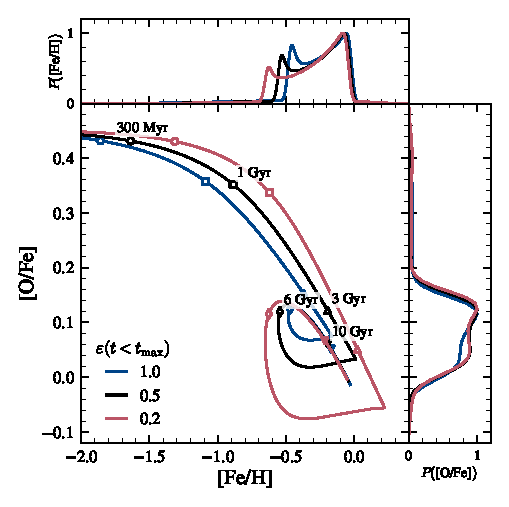
\includegraphics[width=\onecolumn]{src/tex/figures/sfe_prefactor.pdf}
%     \caption{Effect of the SFE timescale pre-factor $\varepsilon$ on abundance tracks and distributions in a one-zone model (see Section \ref{sec:sf-law}). All models are normalized to produce roughly the same ratio of thick to thin disk stars regardless of the value of $\varepsilon$ during the first infall epoch.}
%     \label{fig:sfe-prefactor}
% \end{figure}

In detail, we calculate the star formation efficiency (SFE) timescale $\tau_\star\equiv\Sigma_g/\dot\Sigma_\star$ according to the following:
\begin{equation}
    \label{eq:sf-law}
    \tau_\star = 
    \begin{cases}
        \varepsilon(t) \tau_{\rm mol}(t),   & \Sigma_g \ge \Sigma_{g,0} \\
        \varepsilon(t) \tau_{\rm mol}(t) \Big(\frac{\Sigma_g}{\Sigma_{g,0}}\Big)^{-1/2}, & \Sigma_g < \Sigma_{g,0}
    \end{cases}
\end{equation}
where $\Sigma_{g,0} = 10^8\,{\rm M}_\odot\kpc^{-2}$ and $\tau_{\rm mol}(t)=\tau_{\rm mol,0}(t/t_0)^\gamma$, with $\gamma=1/2$, $t_0=13.8\,{\rm Gyr}$ and $\tau_{\rm mol,0}=2\,{\rm Gyr}$ \citep{leroy_star_2008}. Previous two-infall studies \citep[e.g.,][]{spitoni_galactic_2019,spitoni_galactic_2020,palla_chemical_2020} have adopted a higher SFE during the first infall epoch than the second, which we emulate through the pre-factor $\varepsilon$:
\begin{equation}
    \label{eq:sfe-prefactor}
    \varepsilon(t) = 
    \begin{cases}
        0.5, & t < t_{\rm max} \\
        1.0, & t \ge t_{\rm max}.
    \end{cases}
\end{equation}
A lower value of $\varepsilon(t<t_{\rm max})$ leads to more efficient star formation, and therefore more rapid enrichment, during the first infall epoch. However, the pre-factor has virtually no effect on the overall [O/Fe] distribution because the model is normalized to produce the same thick-to-thin-disk mass ratio regardless of the details of the star formation law. We adopt $\varepsilon(t<t_{\rm max})=0.5$ for consistency with the two-infall literature, though we find $\epsilon(t<t_{\rm max})=0.2$ or $1.0$ produce similar results in one-zone models. To guard against over-correcting the SFE in the early Galaxy, we have tested eliminating either $\varepsilon(t)$ or $\tau_{\rm mol}(t)$ from our SFE prescription in multi-zone models and found no substantial difference to our results.

\subsection{The Gas Supply}
\label{sec:sfh}

We run {\tt VICE} in ``infall mode,'' where we specify the gas infall density $\dot\Sigma_{\rm in}$ and the star formation efficiency (SFE) timescale $\tau_\star\equiv \Sigma_g / \dot\Sigma_\star$ as functions of time at each radius. The gas surface density $\Sigma_g$ and star formation rate $\dot\Sigma_\star$ are calculated from these two inputs as a natural outcome of the time-stepping solution, assuming zero initial gas mass in all zones.

The infall rate as a function of time and galactocentric radius can generically be described by
\begin{equation}
    \label{eq:infall-rate}
    \dot\Sigma_{\rm in}(t,R_{\rm gal}) = A f_{\rm in}(t|R_{\rm gal}) g(R_{\rm gal}),
\end{equation}
where $g(R_{\rm gal})=\Sigma_\star(R_{\rm gal}) / \Sigma_\star(R_{\rm gal}=0)$ is the stellar density gradient, $f_{\rm in}$ is the infall rate over time, and $A$ is a normalization constant. Because we incorporate mass-loaded outflows, $A$ is not analytically solvable, so first we numerically integrate the star formation rate $\dot\Sigma_\star(t,R_{\rm gal})$ and then follow the procedure outlined in Appendix B of \citet{johnson_stellar_2021} to calculate $A$. In short, the infall rate is normalized to produce a total disk stellar mass of $(5.17\pm1.11)\times 10^{10}\,{\rm M}_\odot$ \citep{licquia_improved_2015} and to match the stellar surface density gradient of \citet{bland-hawthorn_galaxy_2016}.

Characteristic of the two-infall scenario, the infall rate is described by two successive, exponentially declining bursts in time. The first infall component induces the formation of the thick disk, and the second component produces the thin disk. At a given galactocentric radius $R_{\rm gal}$, the un-normalized form of the infall rate is
\begin{equation}
    \label{eq:twoinfall-ifr}
    f_{\rm in}(t|R_{\rm gal}) = e^{-t/\tau_1} + H(t-t_{\rm max}) f_{2/1} (R_{\rm gal}) e^{-(t-t_{\rm max})/\tau_2},
\end{equation}
\begin{equation*}
    H(x) \equiv 
    \begin{cases}
        1, & x \ge 0 \\
        0, & x < 0,
    \end{cases}
\end{equation*}
where $\tau_1$ and $\tau_2$ are the first and second infall timescales, respectively, $t_{\rm max}$ is the onset of the second infall and thus the time of maximum gas infall,  $f_{2/1}$ is the ratio of the second infall amplitude to the first, and $H$ is the Heaviside step function. We numerically calculate $f_{2/1}$ for each zone such that the resulting stellar density profile follows a two-component disk, with the surface density ratio of the thick and thin disks given by
\begin{equation}
    f_\Sigma(R) \equiv \frac{\Sigma_1(R)}{\Sigma_2(R)} = f_\Sigma(R_\odot) e^{(R-R_\odot)\cdot(1/R_2 - 1/R_1)}.
\end{equation}
We adopt a thick disk scale radius of $R_1=2.0\kpc$, a thin disk scale radius of $R_2=2.5\kpc$, and a fiducial value for the local surface density ratio of $f_\Sigma(R_\odot)=0.12$ \citep{bland-hawthorn_galaxy_2016}. 

\begin{figure}
    \centering
    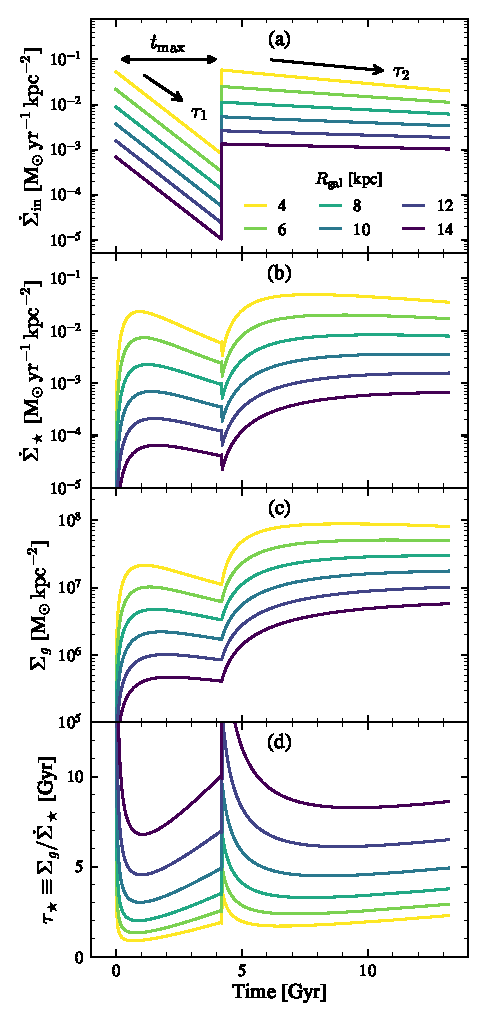
\includegraphics[width=\onecolumn]{figures/star_formation_history.pdf}
    \caption{(a) The infall surface density, (b) the star formation surface density, (c) the gas surface density, and (d) the star formation efficiency timescale as a function of time for our fiducial multi-zone model with $y/Z_\odot=1$. Each panel plots the history for six different zones of width $\delta R_{\rm gal}=0.1\kpc$, color-coded by Galactocentric radius.}
    \label{fig:sfh}
\end{figure}

Figure \ref{fig:sfh} plots the star formation history of several different zones from our fiducial model with $y/Z_\odot=1$. In the inner Galaxy, the infall rate $\dot\Sigma_{\rm in}$ is similar at the start of the first and second infall epochs, and the star formation rate peaks at $t\approx7\,{\rm Gyr}$. In the outer Galaxy, the infall rate at $t_{\rm max}$ is significantly higher than at $t=0$, and the star formation rate is highest at the present day. The star formation efficiency timescale $\tau_\star$ spikes near $t=0$ and $t_{\rm max}$, but otherwise increases throughout the model's duration, reaching a maximum of $\tau_\star\approx2\,{\rm Gyr}$ in the inner disk and $\tau_\star\approx 9\,{\rm Gyr}$ in the outer disk.

The thick-to-thin disk density ratio is especially important for our GCE models as it controls the quantity of gas accreted during each infall epoch. Our fiducial value of $f_\Sigma(R_\odot)=0.12$ is on the low end of literature estimates, which range from $f_\Sigma(R_\odot)\sim0.06-0.6$ \citep[e.g.,][]{gilmore_new_1983,siegel_star_2002,juric_milky_2008,mackereth_age-metallicity_2017,fuhrmann_local_2017}. Previous two-infall studies have adopted a similarly broad range of values (e.g., $f_\Sigma(R_\odot)=0.18$ from \citealt{spitoni_apogee_2021}; $f_\Sigma(R_\odot)=0.4$ from \citealt{spitoni_remind_2024}). We therefore explore values up to $f_\Sigma(R_\odot)=0.5$ in our multi-zone models in Section \ref{sec:multizone-results}.

In most of our models, we assume the infalling gas is pristine (i.e., $Z_{\rm in}=0$). However, the circumgalactic medium (CGM) from which the infalling gas is drawn could be previously enriched, possibly from contributions from Galactic outflows, gas stripped from dwarf galaxies, or from SNe in the halo. The Milky Way's CGM is diffuse, multiphase, and inhomogeneous, making it difficult to study \citep[e.g.,][]{tumlinson_circumgalactic_2017,mathur_probing_2022}; still, recent observations have confirmed the existence of metals at non-Solar abundance ratios in the CGM \citep[e.g.,][]{das_discovery_2019,das_hot_2021,gupta_supervirial_2021}. We investigate models where the infalling gas is pre-enriched, and its metallicity is described by
\begin{equation}
    \label{eq:pre-enrichment}
    Z_{\rm in}(t) = (1 - e^{-t/\tau_{\rm rise}}) Z_\odot 10^{\mathXH_{\rm CGM}}.
\end{equation}
In this case, the metallicity rises from 0 with a timescale $\tau_{\rm rise}=2\,{\rm Gyr}$ and plateaus at $\mathFeH_{\rm CGM}$. Previous GCE studies suggest that some level of enrichment of the infalling gas can improve agreement with observations \citep[e.g.,][]{palla_chemical_2020,johnson_milky_2024,spitoni_remind_2024}. We assume the Solar-scaled metallicity of the accreted gas is the same for all elements (i.e., $\mathXH_{\rm CGM}=\mathOH_{\rm CGM}$).
% We also investigate cases where the CGM is $\alpha$-enhanced, i.e., $\mathOFe_{\rm CGM}>0$.

\subsection{Infall Rate Parameter Selection}
\label{sec:parameter-selection}

\begin{figure*}
    \centering
    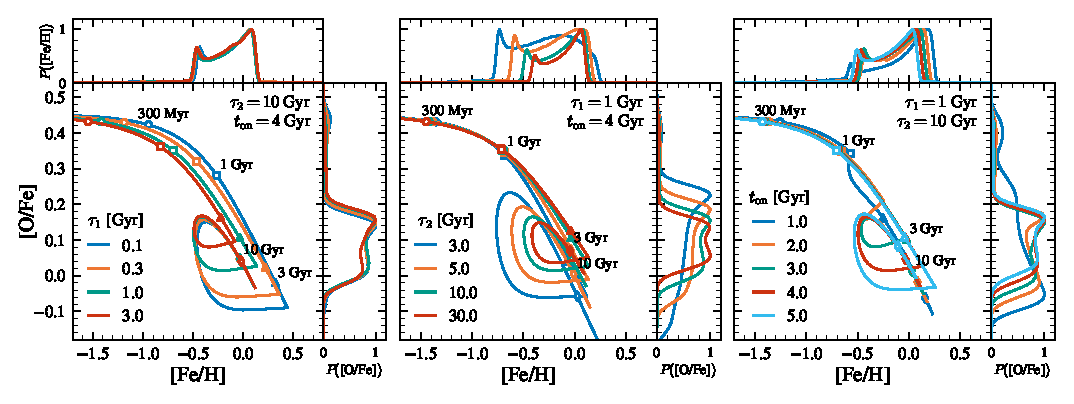
\includegraphics[width=\textwidth]{figures/onezone_params.pdf}
    \caption{Gas abundance tracks in the [O/Fe]--[Fe/H] plane for one-zone chemical evolution models which assume different values for the infall history parameters. In each panel, one parameter is varied according to the legend while the other two are held fixed. The open symbols along each curve mark logarithmic steps in time, as denoted in panel (b). The marginal panels show the corresponding stellar abundance distributions, which are convolved with a Gaussian kernel with a width of 0.02 dex for visual clarity. All models use the same fiducial parameters as the $R_{\rm gal}=8\kpc$ ring in the multi-zone models, with \yZ{1} and $\eta=0.2$. The black lines represent the same set of parameters in each panel.}
    \label{fig:twoinfall-parameters}
\end{figure*}

% The parameters of Equation \ref{eq:infall-rate} have important effects on the chemical evolution of the model. 
% Previous studies of the two-infall model have adopted values for the infall parameters of $\tau_1\sim0.1-1\,{\rm Gyr}$, $\tau_2\sim3-10\,{\rm Gyr}$, and $t_{\rm max}\sim3-5\,{\rm Gyr}$. 
Previous studies have adopted a wide range of parameters for Equation \ref{eq:twoinfall-ifr}. Figure \ref{fig:twoinfall-parameters} illustrates the effect of varying the infall parameters on gas abundance tracks and stellar abundance distributions in a one-zone model with \yZ{1}. The first infall timescale $\tau_1$, shown in panel (a), primarily affects the stellar distribution along the high-$\alpha$ sequence. Though $\tau_1$ has an apparently large effect on the size of the low-$\alpha$ loop, the effect on the stellar abundance distribution of the low-$\alpha$ sequence is quite small due to the low number of stars formed between $t\sim3-6\,{\rm Gyr}$. We adopt $\tau_1=1\,{\rm Gyr}$ for our fiducial value, in line with \citet{spitoni_galactic_2020} but longer than, e.g., \citet{nissen_high-precision_2020} or \citet{spitoni_apogee_2021}, in order to set the peak of the high-$\alpha$ sequence at $\mathOFe\approx+0.3$. 

Panel (b) of Figure \ref{fig:twoinfall-parameters} shows that 
% the second infall timescale $\tau_2$ is the most important parameter to tune in order to reproduce the observed stellar abundance distributions. 
the second infall timescale $\tau_2$ controls the size of the low-$\alpha$ loop, which affects the width of the MDF and the low-$\alpha$ [O/Fe] distribution. A shorter $\tau_2$ produces a bigger loop and therefore a broader [O/Fe] distribution which is skewed to higher [O/Fe], while a longer $\tau_2$ produces a smaller loop, leading to both a narrower low-$\alpha$ sequence and a narrower MDF. We note that our maximum value of $\tau_2=30\,{\rm Gyr}$ is close to a constant infall rate, so a further increase in $\tau_2$ has diminishing effect. Between $\tau_2=3-30\,{\rm Gyr}$, the endpoint of the abundance tracks shifts by $\sim0.2$ dex in [Fe/H] and $\sim0.1$ dex in [O/Fe], which could affect the model's ability to reproduce the present-day abundance of the Solar neighborhood. We adopt a fiducial value of $\tau_2=15\,{\rm Gyr}$ for the Solar neighborhood in order to minimize the size of the loop and width of the low-$\alpha$ [O/Fe] distribution while still approaching Solar [Fe/H] at late times (see further discussion in Section \ref{sec:abundance-distributions}). This value is in line with the infall timescale recovered by \citet{spitoni_galactic_2020}, and similar to the local star formation timescale adopted by \citet{johnson_stellar_2021}, but significantly longer than the timescales found by \citet{nissen_high-precision_2020} and \citet{spitoni_apogee_2021}. 
% In \todo{Section X}, we explore the effect of varying $\tau_2$ with radius in multi-zone models.

In our multi-zone models, we vary the second infall timescale with radius to produce inside-out growth of the disk. Previous multi-zone two-infall studies \citep[e.g.,][]{chiappini_abundance_2001,palla_chemical_2020} scale $\tau_2$ linearly with radius, with $\tau_2\approx1\Gyr$ in the inner disk and $\tau_2=7\Gyr$ at the Solar annulus. This prescription was adopted to match the metallicity distribution of the Solar neighborhood and the bulge in the absence of mass-loaded outflows \citep{romano_mass_2000}. We instead adopt an exponential $\tau_2 - R_{\rm gal}$ relation, with $\tau_2(R_\odot)=15\Gyr$ at the Solar annulus and a scale radius $R_{\tau_2}=7\kpc$. This is similar to the star formation history timescale of \citet{johnson_stellar_2021}, which was based on the  stellar age gradients in Milky Way-like spirals observed by \citet{sanchez_spatially_2020}. We have also run models with a linear prescription and with a uniform value for $\tau_2$ and have found little difference in our key results.

Finally, panel (c) of Figure \ref{fig:twoinfall-parameters} shows that the time of maximum infall $t_{\rm max}$ (c) strongly affects the overall stellar abundance distribution for values $t_{\rm max}\leq2\Gyr$, but in this case the gas tracks do not produce the characteristic abundance loop. For $t_{\rm max}>2\Gyr$, varying $t_{\rm max}$ results in a minor shift to the mean of the MDF and little change to the [O/Fe] distributions, even though the abundance tracks in [O/Fe]--[Fe/H] space appear very different. The value of $t_{\rm max}$ also slightly adjusts the ISM abundance endpoint, as a longer $t_{\rm max}$ means the chemical evolution ``reset'' from the second infall occurs closer to the present day (see discussion in Section \ref{sec:age-abundance}. We adopt a fiducial value of $t_{\rm max}=4.2\Gyr$, i.e. a lookback time of $9\Gyr$, which is generally in line with previous two-infall studies \citep[e.g.,][]{nissen_high-precision_2020,spitoni_galactic_2020,spitoni_apogee_2021}. This ensures that our models are compatible with the median age of the thick disk in the APOKASC-3 catalog of $9.14\pm0.05\Gyr$ \citep{pinsonneault_apokasc-3_2025}. 

The Milky Way's last major merger with the dwarf galaxy, dubbed Gaia Sausage-Enceladus \citep[GSE;][]{belokurov_co-formation_2018,helmi_merger_2018}, has been proposed as an important influence on the transition from the thick disk to the thin disk, as in \citet{spitoni_remind_2024}. Our fiducial value of $t_{\rm max}=4.2\Gyr$ places the start of the formation of the thin disk close to the GSE merger (within uncertainties), which likely occurred $\sim10\Gyr$ ago \citep[e.g.,][]{helmi_merger_2018,gallart_uncovering_2019,naidu_reconstructing_2021,woody_rapid_2025}. However, recent arguments suggest that the GSE merger would not have led to two-infall-like evolution because the mass ratio is too low to produce sufficient dilution \citet{orkney_milky_2025}.

We note that all our models are normalized to produce the same thick-to-thin-disk mass ratio of $f_{\Sigma}(R_\odot)=0.12$ \citep{bland-hawthorn_galaxy_2016} at the Solar annulus regardless of the infall parameters. The high-$\alpha$ sequence appears much less prominent in our [O/Fe] distributions in Figure \ref{fig:twoinfall-parameters} than in the data because the model outputs include only stars which were formed in-situ at the Solar annulus, since they are one-zone models. In our multi-zone models, most of the high-$\alpha$ stars present in the Solar neighborhood have migrated from the inner Galaxy.

\subsection{Stellar Migration}
\label{sec:migration}

This study is not the first to apply a prescription for radial migration to a two-infall GCE model. \citet{spitoni_effect_2015} explored the effect of migration speeds of order $\sim1\,{\rm km}{\rm s}^{-1}$ on the metallicity distribution of the Solar neighborhood. They prescribed some fraction of stars from the inner and outer Galaxy which contribute to the local present-day population based on a constant migration speed, and they also assumed some fraction of stars born in the Solar neighborhood will have migrated elsewhere. This method can improve agreement with the observed local metallicity distribution, but does not scale to abundance distributions across the disk. \citet{palla_mgfe_2022} compared the \citet{spitoni_effect_2015} prescription to the diffusion treatment of \citet{frankel_measuring_2018} and found similar results. Our implementation, described below, affects abundance distributions across the Galaxy, not just at the Solar annulus.

% \citet{spitoni_effect_2015} add a simple radial migration scheme to the model of \citet{spitoni_effects_2011}. They adopt stellar velocities of $\sim 1$ km s$^{-1}$ and assume that some fixed fraction of stars born at a given radius will end up in the Solar vicinity (10\% of those born at 4 kpc and 20\% at 6 kpc). This mimics the results of previous dynamical models such as \citet{minchev_chemodynamical_2013}. They find that by including stellar migration, they are better able to reproduce the high-metallicity tail of the local metallicity distribution, and they also argue that they constrain the migration speed to $0.5 < v < 2$ km s$^{-1}$ based on this tail. Their only point of comparison with data is the local G-dwarf metallicity distribution.

The distance a stellar population born at $R_{\rm form}$ migrates over its age $\tau$ is drawn from a Gaussian centered at 0 with standard deviation
\begin{equation}
    \sigma_{\rm RM} = \sigma_{\rm RM8} \Big(\frac{\tau}{8\,{\rm Gyr}}\Big)^{0.33} \Big(\frac{R_{\rm form}}{8\kpc}\Big)^{0.61},
    \label{eq:radial-migration}
\end{equation}
where we adopt $\sigma_{\rm RM8}=2.68\kpc$ as the fiducial value for the strength of radial migration from \citet{dubay_galactic_2024}. This is smaller than the value of $\sigma_{\rm RM8}=3.6\kpc$ found by \citet{frankel_measuring_2018}, but in Section \ref{sec:age-abundance} we explore the effect of a stronger migration prescription.

All stellar populations are born at the Galactic midplane and are assigned a final midplane distance $z$ drawn from the distribution
\begin{equation}
    p(z|\tau,R_{\rm final}) = \frac{1}{4 h_z} {\rm sech}^2\Big(\frac{z}{2 h_z}\Big)\,
    {\rm \citep{spitzer_dynamics_1942}},
    \label{eq:sech-pdf}
\end{equation}
where $R_{\rm final}$ is the final Galactocentric radius of the stellar population. The width of the distribution $h_z$ is given by
\begin{equation}
    h_z(\tau,R_{\rm final}) = \Big(\frac{0.24\kpc}{e^2}\Big) \exp\Big(\frac{\tau}{7\,{\rm Gyr}} + \frac{R_{\rm final}}{6\kpc}\Big).
    \label{eq:scale-height}
\end{equation}
We note that the final midplane distance is assigned at the end of the model run and therefore does not affect the chemical evolution. The parameters of Equations \ref{eq:radial-migration} and \ref{eq:scale-height} were chosen to fit the stellar migration patterns in the {\tt h277} hydrodynamical simulation \citep{christensen_implementing_2012}. A more complete discussion of the migration scheme and its consequences can be found in Appendix C of \citet{dubay_galactic_2024}.

We note an important distinction between our method and that of \citet{spitoni_effect_2015}: SNe Ia from long-lived progenitors contribute Fe to each zone they migrate through, not just their birth zone. This is important because the median delay time of our SN Ia DTD is $\sim2$ Gyr, for which the width of the migration distribution is $\sigma_{\rm RM}\approx2$ kpc (Equation \ref{eq:radial-migration}). Therefore, a significant fraction of SN Ia progenitors born in a given zone will enrich a different region of the Galaxy.

\section{Multi-Zone Model Results}
\label{sec:multizone-results}

\subsection{Dilution \& Re-enrichment}
\label{sec:age-abundance}

\begin{figure}
    \centering
    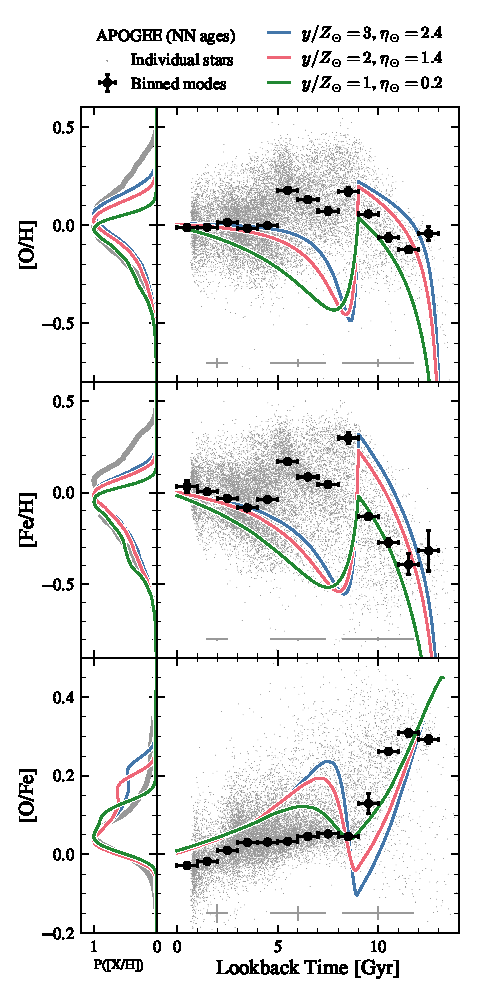
\includegraphics[width=\onecolumn]{figures/gas_abundance_evolution.pdf}
    \caption{The abundance evolution of three one-zone models with different yield sets and outflow mass-loading factors. Table \ref{tab:yields} presents the population-averaged yields for each model. The gray points plot the abundances of APOGEE stars with NN ages from \citet{leung_variational_2023} from the Solar neighborhood ($7\leq R_{\rm gal}<9\kpc$, $0\leq|z|<0.5\kpc$). The black points with error bars indicate the mode of the abundance data in 1 Gyr-wide age bins, and the gray error bars along the bottom of each panel indicate the median age and abundance errors as a function of age.}
    \label{fig:yield-outflow}
\end{figure}

Figure \ref{fig:yield-outflow} shows the mode of the APOGEE [O/H], [Fe/H], and [O/Fe] distributions of mono-age populations in the Solar annulus. As shown by \citet{johnson_milky_2024}, the peak of the MDF is less susceptible to modification by radial migration, making it a more reliable proxy for ISM chemistry at a given lookback time than the mean or median. In agreement with recent work (see discussion in Section \ref{sec:introduction}), the trend with age is interestingly flat. [O/H] and [Fe/H] increase by $0.1-0.2\dex$ in the $\sim6-8\Gyr$ range of ages relative to young stars, likely due to metal-rich stars migrating outward from the inner Galaxy where the surface densities are higher.

We over-plot the ISM abundance evolution in our $y/Z_\odot=1,2,$ and $3$ models at $R_{\rm gal}=8\kpc$ on Figure \ref{fig:yield-outflow} for comparison. The models are in broad agreement with each other and with the data at lookback times of $\lesssim5\Gyr$. At ages of $\sim5-8\Gyr$, the models appear to be in tension with the data, underpredicting the metallicities of the observed stars by up to half an order of magnitude. The low metallicities in the models are a natural consequence of the dilution associated with the second infall event. This discrepancy is potentially mitigated by the higher $y/Z_\odot$ models, which re-enrich more rapidly; signatures of substantial dilution in this scenario may be washed out by age uncertainties. However, these models exacerbate tensions with the age--[O/Fe] relation because the O abundance can grow by a larger factor before enrichment from second-infall SNe Ia becomes important, making the $\alpha$-enhancement from the ensuing starburst more pronounced. When each panel is considered, none of our models provide a good match to these age trends. Figure \ref{fig:yield-outflow} illustrates a point that will arise as a theme throughout the remainder of this paper, which is that the signatures of a substantial dilution event and subsequent re-enrichment, characteristic of the two-infall scenario, are simply not present in the observed age--abundance trends.

% \begin{figure}
%     \centering
%     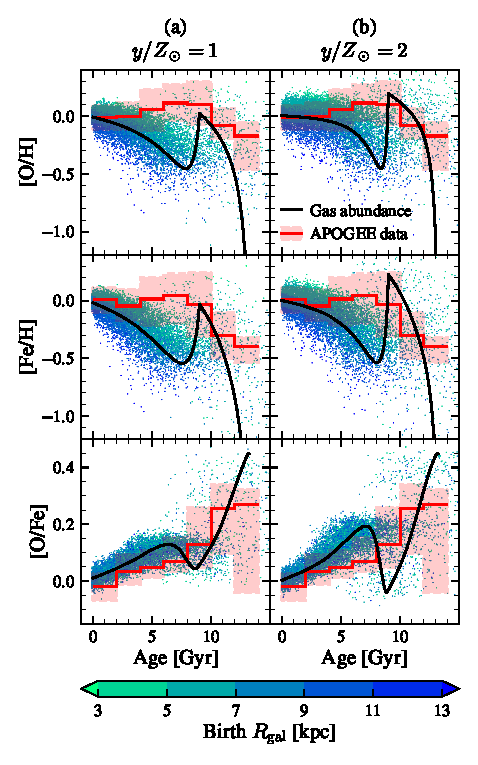
\includegraphics[width=\onecolumn]{figures/abundance_evolution_yields.pdf}
%     \caption{Stellar age--abundance relations predicted by multi-zone models which assume the fiducial parameters with different yield sets and outflow mass-loading factors. Each point represents a stellar population drawn from the Solar neighborhood near the midplane ($7\leq R_{\rm gal}\leq 9\kpc$, $0\leq |z| \leq 0.5\kpc$) and is color-coded by its birth radius. A Gaussian scatter is applied to each point according to the median age and abundance uncertainties in Table \ref{tab:uncertainties}. For visual clarity, we plot only a random mass-weighted sample of \num{10000} points in each panel. The black curve plots the ISM abundance at $R_{\rm gal}=8\kpc$ over time. The red line segments plot the median abundance for APOGEE stars in {2 Gyr}-wide age bins, and the shaded regions represent the 16th--84th percentiles in each bin. Age estimates for APOGEE stars come from \citet{leung_variational_2023}. {\bf Key takeaway:} Both models feature a major dilution event at a lookback time of 9 Gyr, and for model (a) the dilution persists throughout much of the thin disk epoch.}
%     \label{fig:abundance-evolution-yields}
% \end{figure}

% The dilution effect discussed in Section \ref{sec:yields} is clearly seen in our multi-zone model results. Figure \ref{fig:abundance-evolution-yields} shows stellar age--abundance relations predicted by models assuming different yield and outflow scales, \yZ{1} and \yZ{2}, and the fiducial parameters (Table \ref{tab:multizone-parameters}). The \yZ{1} model (column a) shows two clear discrepancies with the \citet{leung_variational_2023} age--abundance relation: a major $\sim0.5$ dex dilution at a lookback time of $\sim9\,{\rm Gyr}$ near where the data show a maximum in [O/H], and noticeable abundance evolution at late times where the data show very little abundance evolution. The evolution of [Fe/H] is similar, but the approach to the final metallicity is slower because of the additional delay imposed by SNe Ia. The \yZ{2} yield set (column b) mitigates both of these issues by shortening the time it takes the ISM metallicity to rebound, producing a much flatter abundance curve at late times. However, model (b) produces a poorer fit to the age--[O/Fe] relation: the decline in [O/Fe] over the thin disk epoch is steeper than the data, especially for ages $\sim4-8\,{\rm Gyr}$. Note that we scatter simulated data points according to the median age and abundance errors in Table \ref{tab:uncertainties}, so the blurring impact of these statistical errors is incorporated in the model. The solid black curve shows the evolution of gas phase abundances at $R_{\rm gal}=8\kpc$. Despite the effects of radial migration and statistical errors, the stellar populations mostly scatter around this gas phase curve, at least for $\tau\lesssim9\Gyr$.

\begin{figure*}
    \centering
    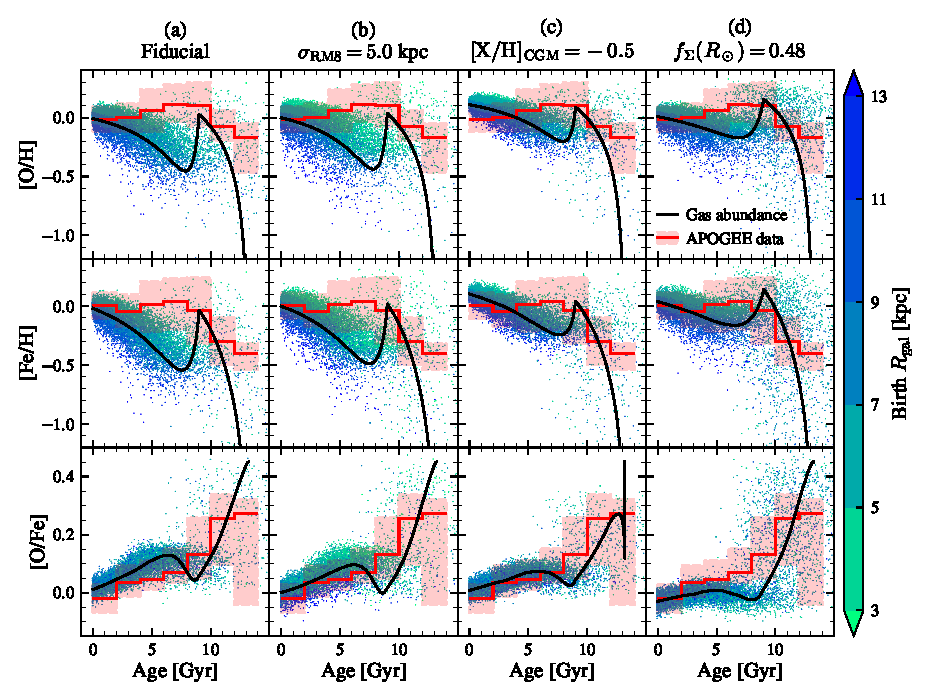
\includegraphics[width=0.9\textwidth]{figures/abundance_evolution_params.pdf}
    \caption{Stellar age--abundance relations predicted by multi-zone models at the \yZ{1} yield scale (see Table \ref{tab:yields}). 
    % The layout is similar to Figure \ref{fig:abundance-evolution-yields}. 
    Each point represents a stellar population drawn from the Solar neighborhood near the midplane ($7\leq R_{\rm gal}\leq 9\kpc$, $0\leq |z| \leq 0.5\kpc$) and is color-coded by its birth radius. A Gaussian scatter is applied to each point according to the median age and abundance uncertainties in Table \ref{tab:uncertainties}. For visual clarity, we plot only a random mass-weighted sample of \num{10000} points in each panel. The black curve plots the ISM abundance at $R_{\rm gal}=8\kpc$ over time. The red line segments plot the median abundance for APOGEE stars in {2 Gyr}-wide age bins, and the shaded regions represent the 16th--84th percentiles in each bin. Age estimates for APOGEE stars come from \citet{leung_variational_2023}.
    Each column shows results from a different multi-zone model: {\bf (a)} our fiducial model with $y/Z_\odot=1$, $\sigma_{\rm RM8}=2.7\kpc$, pristine gas infall, and $f_\Sigma(R_\odot)=0.12$; {\bf (b)} a model with greater radial migration strength $\sigma_{\rm RM8}=5\kpc$; {\bf (c)} a model that assumes the infalling gas has metallicity $\mathOH_{\rm CGM}=\mathFeH_{\rm CGM}=-0.5$; and {\bf (d)} a model with a higher local thick-to-thin disk ratio, $f_\Sigma(R_\odot)=0.5$. {\bf Key takeaway:} Models with pre-enriched infall (c) or a higher thick-to-thin disk ratio (d) reduce the magnitude of the ISM dilution, but neither completely match the observed age--metallicity relation.}
    \label{fig:abundance-evolution-params}
\end{figure*}

Chemical evolution models which assume the \yZ{1} empirical yield scale already struggle to match the local age--metallicity relation, even with a smooth SFH \citep[see also][]{johnson_milky_2024}. The problem is exacerbated in the two-infall case because of the delayed dilution event --- in effect, approach to equilibrium is ``reset'' by the second infall. The dilution of the ISM then gets baked into the stellar abundance record.
Figure \ref{fig:abundance-evolution-params} shows stellar age--abundance relations predicted by models with \yZ{1}. The model with the fiducial parameters (column (a); see Table \ref{tab:multizone-parameters}) shows similar discrepancies with the \citet{leung_variational_2023} age--[O/H] relation as in Figure \ref{fig:yield-outflow}.
% a major $\sim0.5$ dex dilution at a lookback time of $\sim9\,{\rm Gyr}$ near where the data show a maximum in [O/H], and noticeable abundance evolution at late times where the data show very little abundance evolution. 
The evolution of [Fe/H] is similar, but the approach to the final metallicity is slower because of the additional delay imposed by SNe Ia. Note that we scatter simulated data points according to the median age and abundance errors in Table \ref{tab:uncertainties}, so the blurring impact of these statistical errors is incorporated in the model. The solid black curve shows the evolution of gas phase abundances at $R_{\rm gal}=8\kpc$. Despite the effects of radial migration and statistical errors, the stellar populations mostly scatter around this gas phase curve, at least for $\tau\lesssim9\Gyr$.

We next attempt to mitigate the dilution and late-time evolution problems for the empirical (\yZ{1}) yield scale. 
The remaining columns of Figure \ref{fig:abundance-evolution-params} show the effect of varying several parameters for the \yZ{1} model: (b) the strength of radial migration $\sigma_{\rm RM8}$, (c) the metallicity of the infalling gas $\mathXH_{\rm CGM}$, and (d) the local thick-to-thin disk density ratio $f_\Sigma(R_\odot)$.

The observed rise in the median metallicity of stars in the $6-10\Gyr$ age range could be due to radial migration, as those stars were probably not born in-situ, but rather migrated from the metal-rich inner Galaxy \citep{feuillet_age-resolved_2018}. Column (b) of Figure \ref{fig:abundance-evolution-params} presents a model with $y/Z_\odot=1$ and a stronger migration prescription of $\sigma_{\rm RM8}=5\kpc$. As a result, the stars that make up the present-day Solar neighborhood are drawn from a wider range of birth $R_{\rm gal}$, producing a broader abundance distribution at fixed age. Even though this prescription is extreme compared to the estimates of, e.g., \citet{frankel_measuring_2018}, the model still significantly under-predicts the metallicity of $\sim6-10\,{\rm Gyr}$ old stars.

Next, we investigate a model where the infalling gas is enriched to a metallicity $\mathOH=\mathFeH={\rm [X/H]}_{\rm CGM}$ before accreting onto the disk. Column (c) of Figure \ref{fig:abundance-evolution-params} shows results for the case where ${\rm [X/H]}_{\rm CGM}=-0.5$, the highest metallicity allowed by the local low-$\alpha$ population. Pre-enriched infall at this level mitigates but does not completely solve the two discrepancies. The dilution effect of the second infall is reduced to the $\sim0.3$-dex level as the gas which replenishes the Galaxy's reservoir is no longer pristine; however, the width of the stellar abundance distribution at any given age is also reduced since the accreting gas is less chemically different from the ISM, diminishing the effects of dilution. The late-time gas abundance evolution is similar to the fiducial model, but it ends at slightly super-Solar metallicity---an effect which can be compensated by a slightly increased value of $\eta$. This model also narrows the [O/Fe] distribution of mono-age populations (almost all the model stars fall within the $1\sigma$ band of the data), which could be compensated for by stronger radial migration.

Finally, we explore a model where the local thick-to-thin disk surface density ratio is $\sim4$ times larger that the fiducial value, $f_\Sigma(R_\odot)=0.5$. This choice places the ratio higher than most of the constraints from population counts or GCE models (see Section \ref{sec:sfh}). Column (d) of Figure \ref{fig:abundance-evolution-params} shows that requiring a more massive thick disk can reduce the dilution and recent evolution of the ISM, similar to the pre-enriched infall, because more of the gas disk is built up during the first infall phase. The model produces the best agreement with the observed age--[Fe/H] relation (second row). However, agreement with the observed age--[O/Fe] relation is poor, with the model predicting a trend much flatter than observed, underpredicting [O/Fe] by $\sim0.1$ dex in the $\sim6-10\Gyr$ age range.

Overall, no modification to the \yZ{1} model is able to completely overcome the issues that dilution and re-enrichment naturally face when confronted with a flat age--metallicity relation. Pre-enrichment of the accreted gas and a higher disk mass ratio can reduce the discrepancy with the data, but these options introduce new issues in the age--[O/Fe] plane. 

\subsection{Abundance Evolution Across the Disk}
\label{sec:disk-evolution}

\begin{figure*}
    \centering
    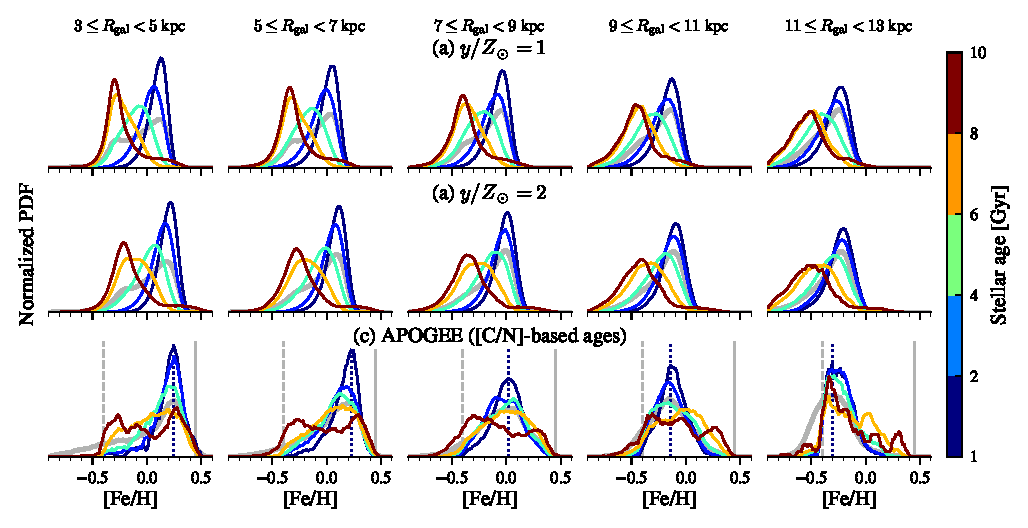
\includegraphics[width=\textwidth]{figures/mdf_evolution.pdf}
    \caption{Evolution of the MDF over time across the Galactic disk. In each panel, normalized stellar [Fe/H] distributions within a {2 kpc}-wide annulus are color-coded by the stellar age range. The gray curve represents the total MDF in each region. Rows (a) and (b) present the distributions from multi-zone GCE models with the fiducial parameters (see Table \ref{tab:multizone-parameters}) at different yield and outflow scales. 
    % For both models we adopt the following non-fiducial parameters: $\mathFeH_{\rm CGM}=-0.7$, $\sigma_{\rm RM8}=3.6$ kpc, and $f_\Sigma(R_\odot)=0.25$. 
    A Gaussian scatter has been applied to each model stellar population in rows (a) and (b) according to the median [C/N]-derived age and abundance uncertainties in Table \ref{tab:uncertainties}. Row (c) presents the distributions from APOGEE DR17 with ages derived from [C/N] abundances (see Section \ref{sec:observational-sample}). The vertical blue dotted lines in row (c) mark the mode of the distribution in the $1-2\kpc$ age bin for reference. Also in row (c), the gray dashed line marks the cut at $\mathFeH>-0.4$ for upper red giant branch and red clump stars, and the gray solid line marks the cut at $\mathFeH<+0.45$ for all stars with [C/N]-based ages. The distributions in all panels are restricted to $0\leq|z|<0.5\kpc$ and boxcar-smoothed with a width of {0.1 dex} for visual clarity. {\bf Key takeaway:} The APOGEE distributions show remarkably little variation in mode [Fe/H] over the past $\sim6-8$ Gyr at all radii, whereas both GCE models predict a steady evolution toward higher [Fe/H] with time.}
    \label{fig:mdf-evolution}
\end{figure*}

The discrepancies between the predicted and observed abundance evolution in the Solar neighborhood discussed in Section \ref{sec:age-abundance} persist across the Galactic disk. Figure \ref{fig:mdf-evolution} shows the evolution of the MDF with age across five radial bins for the \yZ{1} and \yZ{2} models with the fiducial parameters. For the APOGEE sample, we use the [C/N]-derived age estimates due to the larger sample size in the most distant regions of the disk; we limit the comparison to ages in the range $1-10$ Gyr because the [C/N] ages are most reliable in this range, as discussed in Section \ref{sec:observational-sample}. 

The predictions of both models in Figure \ref{fig:mdf-evolution} show a clear trend in [Fe/H] with age at all radii. The MDF shifts consistently toward high metallicity when moving from older to younger stars. The distance between the $1-2\Gyr$ and $2-4\Gyr$ age bins is smaller for the \yZ{2} model because of the faster approach to equilibrium (see also Figure \ref{fig:abundance-evolution-yields}). In the Solar annulus (center column), the peak of the $6-8\Gyr$ old MDF is $0.3\dex$ lower in the \yZ{2} model than observed, and $0.4\dex$ lower in the \yZ{1} model.

In contrast, the APOGEE data show remarkably little evolution in [Fe/H] up to ages of $\sim8\Gyr$ at all radii. Row (c) of Figure \ref{fig:mdf-evolution} shows that the MDF broadens with age, but its peak remains constant across this range. The mode [Fe/H] for the youngest stars (indicated by the vertical blue dotted line) is nearly the same as for the $6-8\Gyr$ old stars. At $R_{\rm gal}<7\kpc$, the MDF skews to lower [Fe/H] more noticeably with age, but its mode does not shift by more than $\sim0.1\dex$. It is difficult to draw conclusions about the outer Galaxy because the mode [Fe/H] is close to the metallicity cut at $\mathFeH>-0.4$ for luminous giants (represented by the vertical gray dashed line), which comprise the majority of stars in the sample at that distance. The remarkable consistency of the MDF over time, the result that motivated the equilibrium scenario proposed by \citet{johnson_milky_2024}, contrasts with the predictions of our fiducial models.

The oldest age bin in Figure \ref{fig:mdf-evolution} shows distinct behavior in both the models and data. The $8-10\Gyr$ age bin spans both the tail end of the thick disk phase and the beginning of the thin disk, so the MDF is bimodal. In the models, the higher peak consists of $>9\Gyr$ old stars (pre-dilution), and the lower peak $8-9\Gyr$ old stars (post-dilution). Intriguingly, the APOGEE MDF in that age bin is also bimodal in all but the outer-most radial bin, with peaks at $\mathFeH\approx-0.3$ and $+0.3$ independent of the location in the Galaxy. While the data and the models show qualitatively similar behavior, they actually represent different populations. In the data, the metal-rich peak are all low-$\alpha$ stars, while the metal-poor peak is the locus of the high-$\alpha$ sequence---a reversal of the model predictions.

\subsection{The Local Abundance Topology}
\label{sec:abundance-distributions}

\begin{figure}
    \centering
    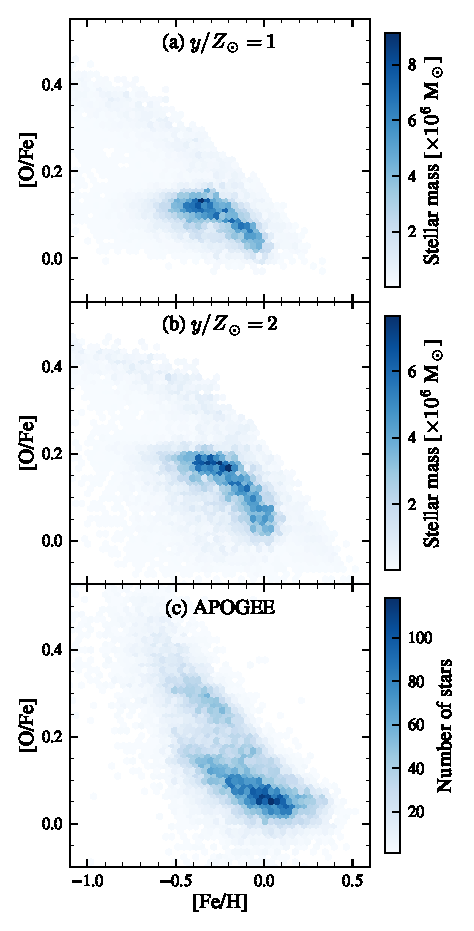
\includegraphics[width=\onecolumn]{figures/ofe_feh_density.pdf}
    \caption{The density of stars in the [O/Fe]--[Fe/H] plane predicted by multi-zone models with (a) $y/Z_\odot=1$ and (b) $y/Z_\odot=2$, and (c) from the APOGEE DR17 catalog. The curves in panels (a) and (b) plot the ISM abundance at the Solar annulus over time, and the alternating black and white segments mark time intervals of {1 Gyr}. The model output has been re-sampled to match the APOGEE stellar $|z|$ distribution, and a Gaussian scatter has been applied to the predicted abundances according to Table \ref{tab:uncertainties}. Stars in all panels are restricted to the region defined by $7\leq R_{\rm gal}< 9\kpc$ and $0\leq|z|<2\kpc$. {\bf Key takeaway:} the two-infall model generically predicts a stellar over-density at intermediate [O/Fe] and low metallicity, which is not observed in APOGEE.}
    \label{fig:ofe-feh-density}
\end{figure}

The two-infall model explains the chemical evolution of the thin disk through the low-$\alpha$ loop (see discussion in Section \ref{sec:parameter-selection}). However, inspection of the marginal [O/Fe] distributions in Figure \ref{fig:ofe-feh-density} reveals a different morphology of the low-$\alpha$ sequence: the two-infall model predicts two peaks in [O/Fe] in the thin disk where the data show only one. The location of the second peak, at intermediate [O/Fe], varies depending on the yields and model parameters (Figure \ref{fig:twoinfall-parameters}), but is always present. This morphology remains essentially consistent in our multi-zone models as well, despite the inclusion of radial mixing and vertical dispersion of stars.

Figure \ref{fig:ofe-feh-density} illustrates the origin of the intermediate-$\alpha$ peak predicted by the two-infall model. Both the models with $y/Z_\odot=1$ and $y/Z_\odot=2$ predict an over-density of stars near the abundance turn-over ($\mathFeH\approx-0.3$, $\mathOFe\approx0.1-0.2$), which is not seen in the APOGEE sample. The local maximum in $dN_\star/d\mathOFe$ comprises stars which formed in the second infall before SN Ia enrichment began to drive down [O/Fe]. This prediction should therefore arise in {\it any} two-infall model regardless of its specific parameters, but its impact can be mitigated through parameter choices that act to compress the distance between the low- and intermediate-$\alpha$ peaks, as in the $y/Z_\odot=1$ model in Figure \ref{fig:yield-outflow} or the models with longer $\tau_2$ in Figure \ref{fig:twoinfall-parameters}.

Additionally, the shape of the low-$\alpha$ sequence predicted the model results (a concave-down ``comma'') is different from the data (a concave-up ``swoosh''). This is a subtle distinction, on the $\sim0.05\dex$ level in [O/Fe]. We have not accounted for the APOGEE selection function in our models, but there is no evident reason for observational effects to produce this difference in morphology. This problem is not unique to the two-infall scenario: it results from the evolution toward the lower right of the [O/Fe]--[Fe/H] plane and has stymied other models as well \citep[e.g.,][]{minchev_chemodynamical_2013,johnson_stellar_2021,prantzos_origin_2023}. The two-infall scenario is otherwise fairly successful at reproducing the local stellar distribution in [O/Fe]--[Fe/H] space.

\subsection{Global Abundance Distributions}
\label{sec:disk-abundances}

\subsubsection{The [O/Fe] Distribution}

% \begin{figure}
%     \centering
%     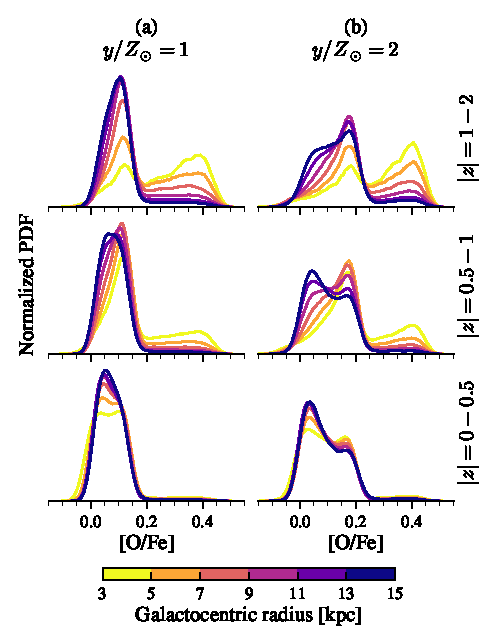
\includegraphics[width=\onecolumn]{src/tex/figures/ofe_distribution_yields.pdf}
%     \caption{Normalized stellar [O/Fe] distributions produced by multi-zone models which assume the fiducial parameters with different yield sets and outflow mass-loading factors. Each row presents stellar distributions within a range of absolute midplane distance $|z|$ reported on the far right, and the vertical scale is consistent across each row. Within each panel, the distributions are color-coded according to the bin in galactocentric radius $R_{\rm gal}$ from which they are drawn. The median APOGEE abundance uncertainties are forward-modeled onto the model outputs (see Table \ref{tab:uncertainties}). For visual clarity, each distribution is smoothed with a box-car of width 0.05 dex. {\bf Key takeaway:} The two-infall model produces an intermediate-[O/Fe] peak that is especially prominent in the \yZ{2} model at mid to high latitudes.}
%     \label{fig:ofe-distribution-yields}
% \end{figure}

% The two-infall model generically predicts {\it three} peaks in the [O/Fe] distribution, which correspond to the high-$\alpha$ sequence, the abundance ``turn-over'' after the second infall, and finally the late-time low-$\alpha$ sequence. We previously noted this feature in \citet{dubay_galactic_2024}. Figure \ref{fig:ofe-distribution-yields} compares [O/Fe] distributions from across the Galactic disk produced by models with the \yZ{1} and \yZ{2} yield sets. We present the distributions in multiple bins of $|z|$ as well as $R_{\rm gal}$ because the observed pattern varies as a function of midplane distance, and because the APOGEE selection function over-emphasizes high-$|z|$, and therefore high-$\alpha$, stars in the full sample \citep[see Figure 5 from][]{vincenzo_distribution_2021}. For model (a) with $y/Z_\odot=1$, the two thin disk peaks are close enough together that they approximate a single peak, especially once observational uncertainties are factored in. With the \yZ{2} yield set, however, there is a $\sim0.2$ dex separation between the low- and intermediate-$\alpha$ peaks thanks to increased efficiency of CCSN element production. As a result, model (b) predicts a high density of stars at $\mathOFe\approx+0.2$ where the data show a relatively low density.

\begin{figure*}
    \centering
    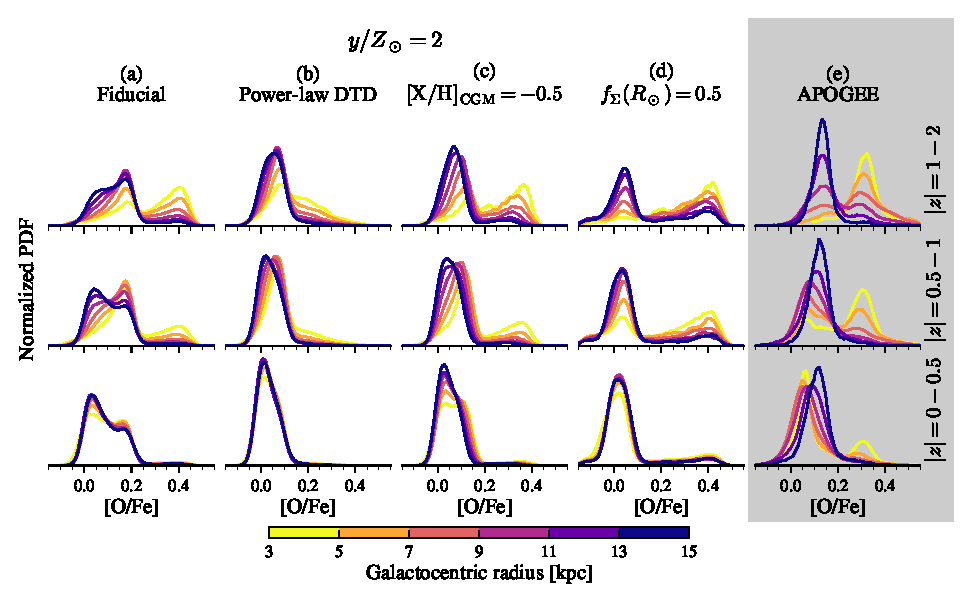
\includegraphics[width=\textwidth]{src/tex/figures/ofe_distribution_params.pdf}
    \caption{Normalized stellar [O/Fe] distributions predicted by multi-zone models with \yZ{2} (a--d) and as observed by APOGEE (e). 
    % The layout is similar to Figure \ref{fig:ofe-distribution-yields}. 
    Each row presents stellar distributions within a range of absolute midplane distance $|z|$ reported on the far right, and the vertical scale is consistent across each row. Within each panel, the distributions are color-coded according to the bin in galactocentric radius $R_{\rm gal}$ from which they are drawn. The median APOGEE abundance uncertainties are forward-modeled onto the model outputs (see Table \ref{tab:uncertainties}). For visual clarity, each distribution is smoothed with a box-car of width 0.05 dex.
    Each column shows the distributions predicted from a different multi-zone model: {\bf (a)} the fiducial model with \yZ{2}, the fiducial DTD, pristine gas infall, and $f_\Sigma(R_\odot)=0.12$
    % (identical to column (b) of Figure \ref{fig:abundance-evolution-yields}); 
    {\bf (b)} a model that adopts a power-law DTD; {\bf (c)} a model that assumes the infalling gas has metallicity $\mathOH_{\rm CGM}=\mathFeH_{\rm CGM}=-0.5$; and {\bf (d)} a model with a higher local thick-to-thin disk ratio, $f_\Sigma(R_\odot)=0.5$. {\bf Key takeaway:} For the \yZ{2} case, pre-enrichment of the accreted gas or a higher thick-to-thin disk ratio can improve the low-$\alpha$ distribution while preserving the high-$\alpha$ peak.}
    \label{fig:ofe-distribution-parameters}
\end{figure*}

In Section \ref{sec:abundance-distributions}, we showed that our high-yield models predict {\it three} peaks in the [O/Fe] distribution, which correspond to the high-$\alpha$ sequence, the abundance ``turn-over'' after the second infall, and finally the late-time low-$\alpha$ sequence. Here, we attempt to mitigate the intermediate peak through several parameter choices.
% In Figure \ref{fig:ofe-distribution-parameters}, we show the result of our attempts to mitigate the intermediate-$\alpha$ peak discrepancy for the \yZ{2} yield set in a few different ways, namely by reducing the size of the thin disk loop seen in panel (b) of Figure \ref{fig:ofe-feh-density}. 
Figure \ref{fig:ofe-distribution-parameters} compares [O/Fe] distributions from across the Galactic disk predicted by models with \yZ{2}. We present the distributions in multiple bins of $|z|$ as well as $R_{\rm gal}$ because the observed pattern varies as a function of midplane distance, and because the APOGEE selection function over-emphasizes high-$|z|$, and therefore high-$\alpha$, stars in the full sample \citep[see Figure 5 from][]{vincenzo_distribution_2021}. The fiducial model (column a) predicts a high density of stars at $\mathOFe\approx+0.2$ where the data show a trough. The peak is most pronounced in the inner disk ($R_{\rm gal}=3-5\kpc$) because of the shorter infall timescale (see Figure \ref{fig:twoinfall-parameters}).

First, we substitute our fiducial SN Ia DTD with a simple power-law,
\begin{equation}
    f_{\rm Ia}^{\rm plaw}(t) = (t/1\,\rm{Gyr})^{-1.1},
    \label{eq:powerlaw-dtd}
\end{equation}
which reduces the median SN Ia delay time from $\sim2\,{\rm Gyr}$ to $\sim0.5\,{\rm Gyr}$. As shown in column (b), this has the intended effect on the low-$\alpha$ sequence, but it also entirely eliminates the high-$\alpha$ peak. \citet{dubay_galactic_2024} discuss in detail why such a DTD is disfavored by Milky Way stellar abundances, and their results hold true for the two-infall model as well.
% In columns (c) and (d) of Figure \ref{fig:ofe-df}, we attempt to mitigate the issue of the intermediate-$\alpha$ peak for the $y/Z_\odot=2$ yield set. Model (c) switches out our fiducial DTD with a power-law DTD, which decreases the timescale for Fe production. However, as shown by \citet{dubay_galactic_2024}, models with a power-law DTD struggle to reproduce the high-$\alpha$ sequence for a wide range of star formation histories, and the results are no different for this two-infall model. 

Next, in model (c) the metallicity of the infalling gas increases to $\mathXH_{\rm CGM}=-0.5$ at late times. We choose this value because if it were any higher, the infalling gas would have higher metallicity than the most metal-poor thin disk stars. This model results in very similar [O/Fe] distributions to the $y/Z_\odot=1$ case. We assume that the infalling gas has $\mathOFe=0$ at all times; an alternate run with $\mathOFe=+0.3$ shifted the distribution towards higher [O/Fe], worsening agreement with observations. 
% In summary, pre-enriched gas infall may be necessary for the two-infall model to match the observed [O/Fe] distribution across the disk.

Finally, in model (d) we increase the local thick-to-thin disk surface density ratio by a factor of 4 to $f_\Sigma(R_\odot)=0.5$. This value means that 1 in 3 stars in the Solar annulus belong to the thick disk and is on the high end of estimates (see Section \ref{sec:sfh}). The result as shown in Figure \ref{fig:ofe-distribution-parameters} is a true bimodal abundance distribution, with a more prominent high-$\alpha$ peak than in the previous models. In summary, either pre-enriched infall or an enhanced disk mass ratio can improve agreement with the observed thin disk abundances for the \yZ{2} case. These parameters also help the model better fit the age--metallicity relation, as shown in Section \ref{sec:age-abundance} for the \yZ{1} case.

\subsubsection{The Best Model}
\label{sec:ofe-feh-best}

\begin{figure*}
    \centering
    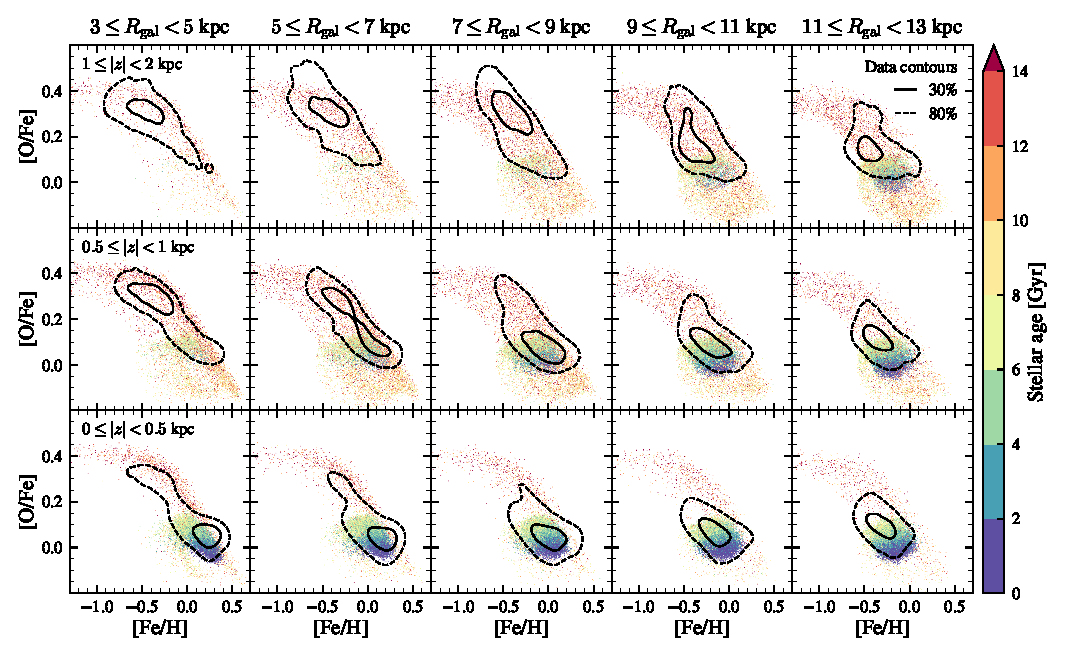
\includegraphics[width=\textwidth]{figures/ofe_feh_best.pdf}
    \caption{Stellar abundance distributions across the disk predicted by our best multi-zone model, with \yZ{2}, ${\rm [X/H]}_{\rm CGM}=-0.7$, $f_\Sigma(R_\odot)=0.25$, $\sigma_{\rm RM8}=3.6\kpc$, and $\eta_\odot=1.8$. Each panel presents a random mass-weighted sample of \num{10000} stellar populations that are drawn from the given ($R_{\rm gal}$, $|z|$) bin and color-coded by age. A Gaussian scatter is applied to each point according to the median age ($\tau_{\rm [C/N]}$) and abundance uncertainties in Table \ref{tab:uncertainties}. The solid and dashed contours enclose 30\% and 80\%, respectively, of the APOGEE data in each region. {\bf Key takeaway:} The predicted distribution from the two-infall model lines up with the APOGEE distribution close to the midplane, but agreement is worse at higher latitudes and in the outer Galaxy.}
    \label{fig:ofe-feh-best}
\end{figure*}

Motivated by the results of the previous sections, we construct a model which attempts to solve all of the issues that have been outlined thus far. Our ``best attempt'' model uses the \yZ{2} yield set to flatten the local age--metallicity relation (Figure \ref{fig:abundance-evolution-yields}), pre-enriched infall at the level of $\mathXH_{\rm CGM}=-0.7$ to reduce the dilution at $t_{\rm max}$ (Figure \ref{fig:abundance-evolution-params}), slightly stronger outflows with $\eta_\odot=1.8$ to maintain the local equilibrium at Solar metallicity, moderately stronger radial migration with $\sigma_{\rm RM8}=3.6\kpc$ to widen the local metallicity dispersion (Figure \ref{fig:abundance-evolution-params}), and a greater local disk ratio $f_\Sigma(R_\odot)=0.25$ to reduce the width of the low-$\alpha$ distribution and beef up the high-$\alpha$ sequence (Figure \ref{fig:ofe-distribution-parameters}). Our choices for $\mathXH_{\rm CGM}$, $\sigma_{\rm RM8}$, and $f_\Sigma(R_\odot)$ are more moderate, and we believe more realistic, than in previous sections to avoid extreme effects resulting from the combination of these parameters. We stress that our focus is on qualitative rather than quantitative agreement with the data, and thus we do not attempt to find the optimal set of parameters through methods such as MCMC.

Figure \ref{fig:ofe-feh-best} shows the stellar [O/Fe]--[Fe/H] distributions in different ranges of $R_{\rm gal}$ and $|z|$ color-coded by age as predicted by the best model. This model is generally successful at reproducing the observed distribution, especially in the inner Galaxy and close to the midplane. However, the predicted high-$\alpha$ sequence has a significant presence even in the outer Galaxy---likely a consequence of the stronger migration prescription and higher thick-to-thin disk ratio. In general, the predicted distributions do not align with the data as well at large midplane distances ($1\leq|z|<2\kpc$), but this may partly be due to our prescription for vertical heating (see Section \ref{sec:migration}).

The model makes two notable predictions about the age--abundance distributions. First, there is a population of $\sim8-9\Gyr$ old stars at sub-Solar [O/Fe], especially at $|z|\ge0.5\kpc$, formed immediately after the second infall during a period of rapid chemical evolution. These stars form a small percentage of the overall distribution \citep[see also Figure 11 from][]{spitoni_remind_2024} but in this case they occupy a unique portion of the abundance space. A longer $\tau_1$ could shift this population to higher [O/Fe] where it would be obscured by the rest of the low-$\alpha$ sequence (see Figure \ref{fig:twoinfall-parameters}). Second, the stars born at the tail end of the thick and thin disk epochs are adjacent to each other in abundance space, meaning the two-infall model predicts a bimodal age distribution for metal-rich stars.

\subsection{Local Age Patterns}

\begin{figure*}
    \centering
    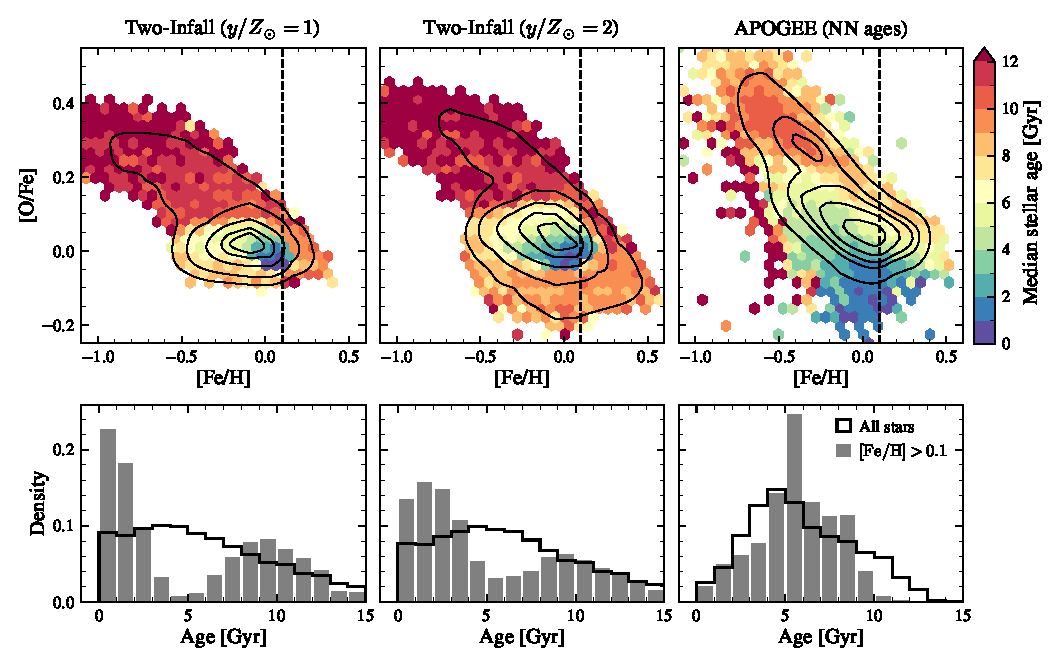
\includegraphics[width=\textwidth]{figures/lmr_ages.pdf}
    \caption{{\it Top:} The median stellar age as a function of [O/Fe] and [Fe/H] in the Solar annulus ($7\leq R_{\rm gal}<9\kpc$, $0\leq|z|<2\kpc$). The left and center panels plot the output of our best two-infall models, with \yZ{2}, ${\rm [X/H]}_{\rm CGM}=-0.7$, $f_\Sigma(R_\odot)=0.25$, and $\sigma_{\rm RM8}=3.6\kpc$. The model output has been re-sampled to match the APOGEE stellar $|z|$ distribution, and a Gaussian scatter has been applied to the abundances and ages according to Table \ref{tab:uncertainties}. The right panel plots the results from APOGEE using the \citet{leung_variational_2023} age catalog. The contours indicate the density of stars in the [Fe/H]--[O/Fe] plane, and the vertical dashed line denotes the boundary for locally metal-rich (LMR) stars.
    {\it Bottom}: Stellar age distributions in the Solar annulus for all stars (black) and LMR stars (gray). The left and center panels plot the mass-weighted age distributions predicted by the models after forward-modeling age uncertainties, and the right panel plots the \citet{leung_variational_2023} ages for APOGEE stars.
    {\bf Key takeaway:} The two-infall model predicts a fundamentally different age pattern than what is observed, especially for LMR stars.}
    \label{fig:lmr-ages}
\end{figure*}

The two-infall model makes a fundamental prediction about the local stellar age distribution: the most metal-rich stars born in-situ in any region of the Galaxy should come from the metal-rich tail of the first infall sequence, and are therefore older than all of the thin disk stars. As noted in the previous Section, this prediction is apparent in any of the panels in Figure \ref{fig:ofe-feh-best}, especially where $|z|<0.5\kpc$. We investigate this prediction further here.

The top row of Figure \ref{fig:lmr-ages} presents the median stellar age as a function of [O/Fe] and [Fe/H] for two multi-zone models and in APOGEE. While the models predict a fairly accurate distribution of stars in abundance space, especially for the low-$\alpha$ population, the stellar age patterns are starkly different. In both the \yZ{1} and \yZ{2} models, there is a sharp divide in the median stellar age when moving from the thick disk ($\tau\ge9\Gyr$) to the thin disk ($\tau\lesssim5\Gyr$). The \yZ{2} model also predicts that the stars with the lowest [O/Fe] should be $\sim8-9\Gyr$ old, while these are some of the youngest stars in APOGEE. The latter issue can be mitigated by adjusting the parameters of the first infall, as discussed in the previous Section, but the former is not solved so easily.

We further highlight the discrepant age patterns in the bottom panels of Figure \ref{fig:lmr-ages}, which compare the overall stellar age distribution against that of the locally metal rich (LMR) stars, defined here as $\mathFeH\ge+0.1$.\footnote{
    While the amplitude of the peaks is sensitive to the precise location of the LMR cutoff, the dearth of intermediate-age stars is robust to adjustments of $\pm0.05\dex$.
} For APOGEE, the distributions are similar, both peaking near $\sim5\Gyr$, although very few of the LMR stars have ages $\gtrsim10\Gyr$. Our two-infall models predict an overall age distribution that is similar to the data, but both models predict a distinctly bimodal age distribution for LMR stars. The two populations reflect the metal-rich endpoints of the two successive infall epochs. The trough between the modes lies at $\sim5\Gyr$ for both models, right where the APOGEE distribution peaks. It is difficult to predict a unimodal age distribution with the available parameter space. A dearth of intermediate-age, high-metallicity stars is a natural outcome of a substantial dilution event, which is a defining feature of the two-infall scenario. None of the adjustments that we explored in Figure \ref{fig:abundance-evolution-params} substantially increase the proportion of intermediate-age stars.

\section{Discussion}
\label{sec:discussion}

% \todo{Summary of problem: the two-infall model is boxed in by data.}
Our results show that the APOGEE stellar age catalogs pose several challenges to the two-infall scenario. The [O/Fe] distribution was the observable with the easiest discrepancy to resolve using the parameter space we explored, either by pre-enrichment of the accreted gas or a higher thick-to-thin disk mass ratio. These parameters also allowed us to mitigate, but not completely resolve, the issues with the age--abundance relations caused by dilution. The predicted age distributions could not be reconciled with the data using any of the variations we explored. In the remainder of this section, we discuss other parameters explored by previous studies as well as further extensions to the two-infall model.

\subsection{Third Accretion Episode}

Motivated by evidence of a recent period of enhanced star formation \citep[e.g.,][]{ruiz-lara_recurrent_2020}, \citet{spitoni_beyond_2023} and \citet{palla_mapping_2024} extended the two-infall model with a recent $(\lesssim3\Gyr)$ third accretion episode. \citet{spitoni_beyond_2023} argued that the gas dilution resulting from the third infall could explain the population of young, metal-poor stars discovered in {\it Gaia} DR3 \citep{recio-blanco_gaia_2023}, in contrast to the two-infall model of \citet{spitoni_apogee_2021} which predicted a present-day gas metallicity of ${\rm [M/H]}\approx+0.3$ in the Solar neighborhood. \citet{palla_mapping_2024} were similarly motivated by the finding that open clusters with ages $<1\Gyr$ have similar metallicity to those with ages $>3\Gyr$, while the classical two-infall model predicted a steady increase in metallicity over time. However, \citet{palla_mapping_2024} invoke a less massive infall, producing a milder dilution event, than \citet{spitoni_beyond_2023}.

The flat AMR from both stellar age catalogs is even more restrictive of a recent dilution event because of the smaller age uncertainties for younger stars. Figure \ref{fig:yield-outflow} illustrates that the mode and overall distribution of [O/H] has evolved very little over the past $\sim5$ Gyr. Some combination of metal-rich accretion or radial gas flows might reduce the amount of dilution predicted by a recent accretion episode, but the parameter space is tightly constrained by the stellar age data.

\subsection{Radial Gas Flows}
\label{sec:radial-flows}

Radial gas flows are a potential alternative to the outflow prescription that we use in this paper. Within the two-infall paradigm, \citet{spitoni_effects_2011} found that inward flow velocities of a $\sim$ few $\kms$ can steepen the predicted radial metallicity gradient to match observations. Similarly, \citet{palla_chemical_2020,palla_mapping_2024} used an inward flow with a speed of $\sim1\kms$ to reproduce the observed radial metallicity profile in the absence of Galactic outflows. Johnson et al. (2025, in preparation) considered several possible scenarios for the processes that drive radial gas flows. Their findings support these previous arguments that radial gas flows should regulate the overall metal abundance and radial gradient, even beyond the two-infall scenario.

In our models, the outflows regulate the overall metallicity in a radially dependent manner, which \citet{johnson_milky_2024} demonstrated to improve agreement with age trends across the Galactic disk. Johnson et al. (2025, in preparation) found similar results for radial gas flows with velocities that are relatively constant in both Galactocentric radius and time. At least one radial gas flow scenario therefore has similar effects on metal enrichment as our outflow prescription. However, the outflow is simpler in implementation; we can simply adjust the mass loading factors up or down in combination with a given scale of yields. This approach allows us to easily consider models that predict metallicity to evolve on different timescales but reach similar abundances at the present day (see, e.g., Figure \ref{fig:yield-outflow}). A radial gas flow requires at least one assumption about the processes that drive the flow and generally do not afford the same level of flexibility. We have therefore focused on models with outflows in this paper for the sake of simplicity, and we clarify that some, but not all, radial gas flow models should have similar effects.

\subsection{Star Formation Hiatus}
\label{sec:sfe-hiatus}

\begin{figure}
    \centering
    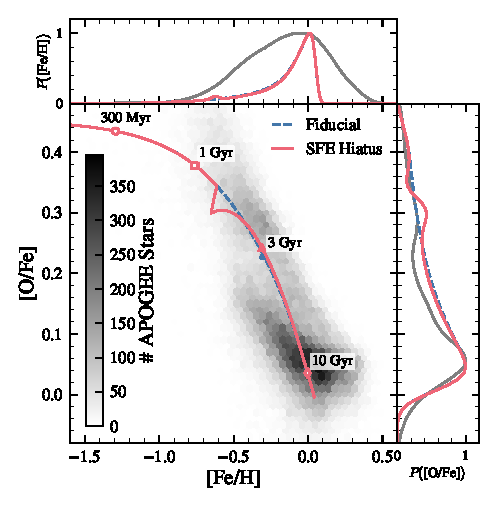
\includegraphics[width=\onecolumn]{figures/onezone_sfe_hiatus.pdf}
    \caption{Abundance tracks and distributions from one-zone models which experience an efficiency-driven starburst. The blue dashed curve represents the fiducial model that has an exponentially declining infall rate and constant star formation efficiency timescale $\tau_\star=2\,{\rm Gyr}$. The red solid curve plots the output of a model which experiences an enhancement of $\tau_\star$ by a factor of 10, for a duration of 200 Myr, starting at $t=1.4\,{\rm Gyr}$. Both models assume the \yZ{2} yield set, with $y_{\rm Fe}^{\rm Ia}$ reduced by 20\% to better match the model endpoint with the data, and $\eta=1.4$. The greyscale histogram presents the number density of APOGEE stars in the Solar annulus ($7\leq R_{\rm gal}\leq 9\kpc$, $0\leq|z|\leq2\kpc$) in [O/Fe]--[Fe/H] space, and the gray histograms in the marginal panels show the APOGEE stellar abundance distributions.}
    \label{fig:onezone-sfe-hiatus}
\end{figure}

The two-infall model falls into the broader category of GCE models which reproduce the $\alpha$-bimodality by halting or severely limiting star formation for some duration. For the two-infall model, this phase of low star formation immediately precedes the second infall epoch and is due to the relatively short timescale of the first infall epoch. However, as we have shown, the dilution of the ISM resulting from the second infall poses a challenge when comparing to age--abundance data.

A bursty infall history is not the only way to produce a gap in the star formation history. \citet{beane_rising_2024} present a simulated galaxy from the Illustris TNG50 suite that exhibits MW-like bimodality. They argue that the $\alpha$-bimodality is brought on by a brief ($\sim300\,{\rm Myr}$) quiescent period caused by bar formation. The virial mass of their galaxy grows steadily throughout this period, unlike in our two-infall model where the mass grows by a factor of \todo{X} during the 1 Gyr following the second infall.

While our semi-analytic model does not include a Galactic bar, we can explore the effects of a star formation hiatus by artificially boosting the SFE timescale $\tau_\star$ for a period of time. Figure \ref{fig:onezone-sfe-hiatus} illustrates the effect of this SFE-driven hiatus in a one-zone model with an exponentially declining infall rate. During the quiescent period, the [O/Fe] ratio slowly declines due to the delayed contribution of Fe from SNe Ia. Meanwhile, the gas mass continues to increase even as star formation is suppressed. When $\tau_\star$ is lowered at the end of the quiescent period, the high gas mass sparks a moderate star formation burst which causes stellar abundances to ``pile up'' at similar [O/Fe] values. The trough between the high- and low-$\alpha$ sequences results from the star formation returning to pre-quiescence behavior.

Our simple hiatus model offers a few parameters which control the chemical evolution. The onset time of the SFE hiatus controls the position of the high-$\alpha$ sequence: a later onset places the peak at lower [O/Fe]. The duration of the star formation hiatus and the $\tau_\star$ enhancement factor control the strength of the high-$\alpha$ peak.

The parameters of the SFE hiatus in Figure \ref{fig:onezone-sfe-hiatus} were chosen to match the APOGEE stellar [O/Fe] distribution as closely as possible. However, there are some differences in detail, such as the dearth of stars at $\mathOFe\approx+0.35$ due to the star formation hiatus. We intend this model to illustrate another path to reproducing the $\alpha$-bimodality. Most of the high-$\alpha$ stars present in the Solar annulus have likely migrated from the inner Galaxy, where perhaps this SFE-driven hiatus was concentrated.

\section{Summary \& Conclusions}
\label{sec:conclusions}

We have compared the predictions of the two-infall scenario against abundance data from APOGEE DR17 supplemented with age estimates using two different methods. We ran multi-zone GCE models at two different yield scales with prescriptions for radially-dependent outflows and stellar migration. While the two-infall scenario can explain the distinct high- and low-$\alpha$ sequences, it faces challenges in matching the age--abundance structure of the full disk. We explored multiple parameter modifications to bring the model predictions closer to the data, including the yield scale, radial migration strength, metallicity of the accreted gas, thick-to-thin disk mass ratio, and the SN Ia DTD. Our conclusions are as follows:

\begin{itemize}
    \item The large quantity of pristine gas accreted in the Solar neighborhood during the second infall phase rapidly dilutes the ISM metallicity by $\sim0.5$ dex. Models with low nucleosynthetic yields (\yZ{1}) remain at sub-Solar metallicity until the present day, in stark contrast to the observed local age--metallicity relation. Models with higher yields and outflows approach the present-day metallicity more rapidly, while pre-enriched infall can reduce the magnitude of the dilution (but not eliminate it entirely). %This issue can be mitigated with higher yields and outflows, but not by pre-enriched infall or radial migration.
    \item For metal-rich stars, the two-infall model predicts a sharp divide in the stellar age distribution between the thick and thin disk populations. In contrast, the data show a smooth gradient between the oldest and youngest stars, with most of the metal-rich stars having intermediate ages.
    \item The ``turn-over'' in the evolution of [O/Fe] following the second infall produces a double-peaked low-$\alpha$ sequence with a fundamentally different abundance structure than observed, especially for models with higher yields. A low yield set (\yZ{1}) coupled with lower outflows, or pre-enrichment of the infalling gas, can bring the stellar [O/Fe] distributions more in line with the data. The parameter space is nonetheless restricted by the need to suppress this feature.
    \item Our models predict that the MDF evolves to higher metallicity over time throughout the disk. This contrasts with the APOGEE data, which show very little change in the mode over the past $\sim6-8$ Gyr.
    % \item The equilibrium scenario of chemical evolution, if correct, places stricter limits on the two-infall model than other evolutionary models.
    \item Adjusting the strength of radial migration naturally affects the scatter in the age--metallicity relation but does not affect the median age.
\end{itemize}

The apparent age-independence of stellar abundances in the disk places considerable restrictions upon the two-infall parameter space because it predicts a substantial dilution event at the start of the thin disk epoch. If the equilibrium scenario of \citet{johnson_milky_2024} is correct, then it restricts the two-infall scenario more than other GCE models. Restrictions on the two-infall scenario also translate more broadly to other merger-dominated SFHs, which must explain the MW's $\alpha$-bimodality without significantly diluting the metallicity of the ISM.

\section*{Acknowledgements}

\todo{Personal acknowledgements.}

LOD and JAJ acknowledge support from National Science Foundation grant no.\ AST-2307621. JAJ and JWJ acknowledge support from National Science Foundation grant no.\ AST-1909841.
LOD acknowledges financial support from an Ohio State University Fellowship.
JWJ acknowledges financial support from an Ohio State University Presidential Fellowship and a Carnegie Theoretical Astrophysics Center postdoctoral fellowship. \todo{Update grants and fellowships.}

Funding for the Sloan Digital Sky 
Survey IV has been provided by the 
Alfred P.\ Sloan Foundation, the U.S.\ 
Department of Energy Office of 
Science, and the Participating 
Institutions. 

SDSS-IV acknowledges support and 
resources from the Center for High 
Performance Computing  at the 
University of Utah. The SDSS 
website is \url{www.sdss4.org}.

SDSS-IV is managed by the 
Astrophysical Research Consortium 
for the Participating Institutions 
of the SDSS Collaboration including 
the Brazilian Participation Group, 
the Carnegie Institution for Science, 
Carnegie Mellon University, Center for 
Astrophysics | Harvard \& 
Smithsonian, the Chilean Participation 
Group, the French Participation Group, 
Instituto de Astrof\'isica de 
Canarias, The Johns Hopkins 
University, Kavli Institute for the 
Physics and Mathematics of the 
Universe (IPMU) / University of 
Tokyo, the Korean Participation Group, 
Lawrence Berkeley National Laboratory, 
Leibniz Institut f\"ur Astrophysik 
Potsdam (AIP),  Max-Planck-Institut 
f\"ur Astronomie (MPIA Heidelberg), 
Max-Planck-Institut f\"ur 
Astrophysik (MPA Garching), 
Max-Planck-Institut f\"ur 
Extraterrestrische Physik (MPE), 
National Astronomical Observatories of 
China, New Mexico State University, 
New York University, University of 
Notre Dame, Observat\'ario 
Nacional / MCTI, The Ohio State 
University, Pennsylvania State 
University, Shanghai 
Astronomical Observatory, United 
Kingdom Participation Group, 
Universidad Nacional Aut\'onoma 
de M\'exico, University of Arizona, 
University of Colorado Boulder, 
University of Oxford, University of 
Portsmouth, University of Utah, 
University of Virginia, University 
of Washington, University of 
Wisconsin, Vanderbilt University, 
and Yale University.

This work has made use of data from the European Space Agency (ESA) mission
{\it Gaia} (\url{https://www.cosmos.esa.int/gaia}), processed by the {\it Gaia}
Data Processing and Analysis Consortium (DPAC,
\url{https://www.cosmos.esa.int/web/gaia/dpac/consortium}). Funding for the DPAC
has been provided by national institutions, in particular the institutions
participating in the {\it Gaia} Multilateral Agreement.

% From the Center for Belonging and Social Change, https://cbsc.osu.edu/about-us/land-acknowledgement
We would like to acknowledge the land that The Ohio State University occupies is the ancestral and contemporary territory of the Shawnee, Potawatomi, Delaware, Miami, Peoria, Seneca, Wyandotte, Ojibwe and many other Indigenous peoples. Specifically, the university resides on land ceded in the 1795 Treaty of Greeneville and the forced removal of tribes through the Indian Removal Act of 1830. As a land grant institution, we want to honor the resiliency of these tribal nations and recognize the historical contexts that has and continues to affect the Indigenous peoples of this land.

\software{\vice \citep{johnson_impact_2020}, Astropy \citep{astropy_collaboration_astropy_2013,astropy_collaboration_astropy_2018,astropy_collaboration_astropy_2022}, scikit-learn \citep{pedregosa_scikit-learn_2011}, SciPy \citep{virtanen_scipy_2020}, Matplotlib \citep{hunter_matplotlib_2007}.}

\appendix

\section{Reproducibility}
\label{app:reproducibility}

\todo{Blah.}

\bibliography{references}

\end{document}
